\section{Results}
\label{sec:results}
We organize the presentation of our findings by topic, including how users
\emph{perceive} (\Cref{sec:perception}), \emph{manage} (\Cref{sec:manage}),
and \emph{wish to improve} (\Cref{sec:improve}) onion services.  We interleave the
results from our online survey with our interviews, focusing primarily on our
survey data but bringing up anecdotes and findings from our interviews as
appropriate.

\subsection{User Perceptions of Onion Services}
\label{sec:perception}

\subsubsection{Mental Models of Onion Services}


Our participants perceived onion services’ definition, the way they work, as well as their content in many different ways and from different perspectives. However, almost half of our interviewees (8/17) seemed to be confused about onion services, they were not sure how they function, how to describe them and they did not understand how onion services protect them. 

Above all, according to the majority of our interviewees (9/17) onion services enable the user to access Web content in anonymous manner. Moreover, 3 interview participants stressed that such protection is not only for visitors but also for people providing these services. One of the interviewees was particularly curious how OS facilitate anonymous purchases and pointed out usage of CryptoMoney as one of the characteristics of Onion Links: \textquote[P11]{I was reading the other day about how to use some the web to buy things because I was interested to understand how you can do that, to buy like abortion pills or things like that.} Another two participants also mentioned possibility of participating in illegal actions such as drug trade and credit card data sale. Some of our interviewees did not distinguish disguising their \textsc{ip}  address from disguising their real-world identity and instead used the umbrella term of “anonymity” to refer
to both concepts. This conflation of concepts paints
an incomplete picture of the security and privacy guarantees
that the Tor network provides, further illustrated
by one interview participant’s question: \textquote[P07]{What's the point of going to Facebook using onion services when
their business model is still about collecting your data?}

Six interviewees stated that onion links are related to extra layers of protection, which sketch\footnote{All sketches are available online at
\url{https://nymity.ch/onion-services/mental-models/}.} that we can see on \Cref{fig:os-sketch} and explanation of participant P03 illustrates well:   “I think it's kind of to do with the different hops that you build different layers of making it difficult to find out who this person is. “. It corresponds to the notion of protective feature of OS to which 5 interviewees related to when describing onion links.


\begin{figure}[!ht]
    \centering
        \centering
        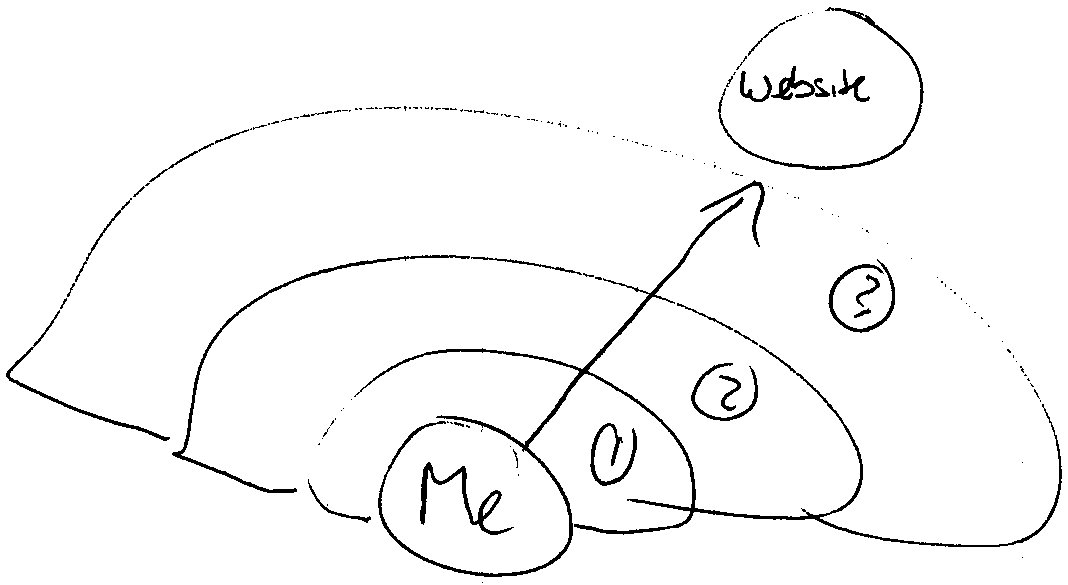
\includegraphics[width=0.8\linewidth]{figures/p03-os-sketch-kopia2.jpg}
        \caption{Sketch of interviewee's (P03) mental model of Onion Services. The participant referred to extra layers of protection.}
        \label{fig:os-sketch}
\end{figure}

More interview participants (5) saw the connection between Tor and onion services and stated OS are to be accessed through Tor than those that did not see any connection between those two (1).  While the participants that saw this connection between Tor and onionservices  stated  that  onion  services are to be accessed through Tor, we can  see that this knowledge is notwidespread, as evidenced by our findings in analyz-ing the root DNS data described in \Cref{sec:root_data}.We found 15,471 correctly-formatted onion domains\footnote{Note that these may not all correspond to real onion sites, as some-one could have entered a bogus onion domain name into a browser; un-fortunately, there is no way for us to evaluate the validity of each oniondomain.} in the dataset,  indicating that Internet users are attempting tovisit an onion domain in a non-Tor browser.

Another interesting assumption was made by interview participant P07 – he claimed that OS 

“It's essentially the Tor project being able to make their technology available to more commercial clients, having that option be available to them. For me, it's all about trying to scale what they're doing.”, thinking about more economic traits of OS than other participants, whereas P08 considered OS as “Internet without hyperlinks”.

Four interviewees stated that OS work in a similar manner to Tor but what is interesting, the same 4 participants also thought that encryption is a little bit different than in Tor, which we can see on \Cref{fig:toros-sketch}. Furthermore, four interviewees described the way of how OS work referring to the encryption of data onto the end point and 3/17 to the fact that last point of the chain of the encryption is an onion link. 


\begin{figure}[!ht]
        \centering
        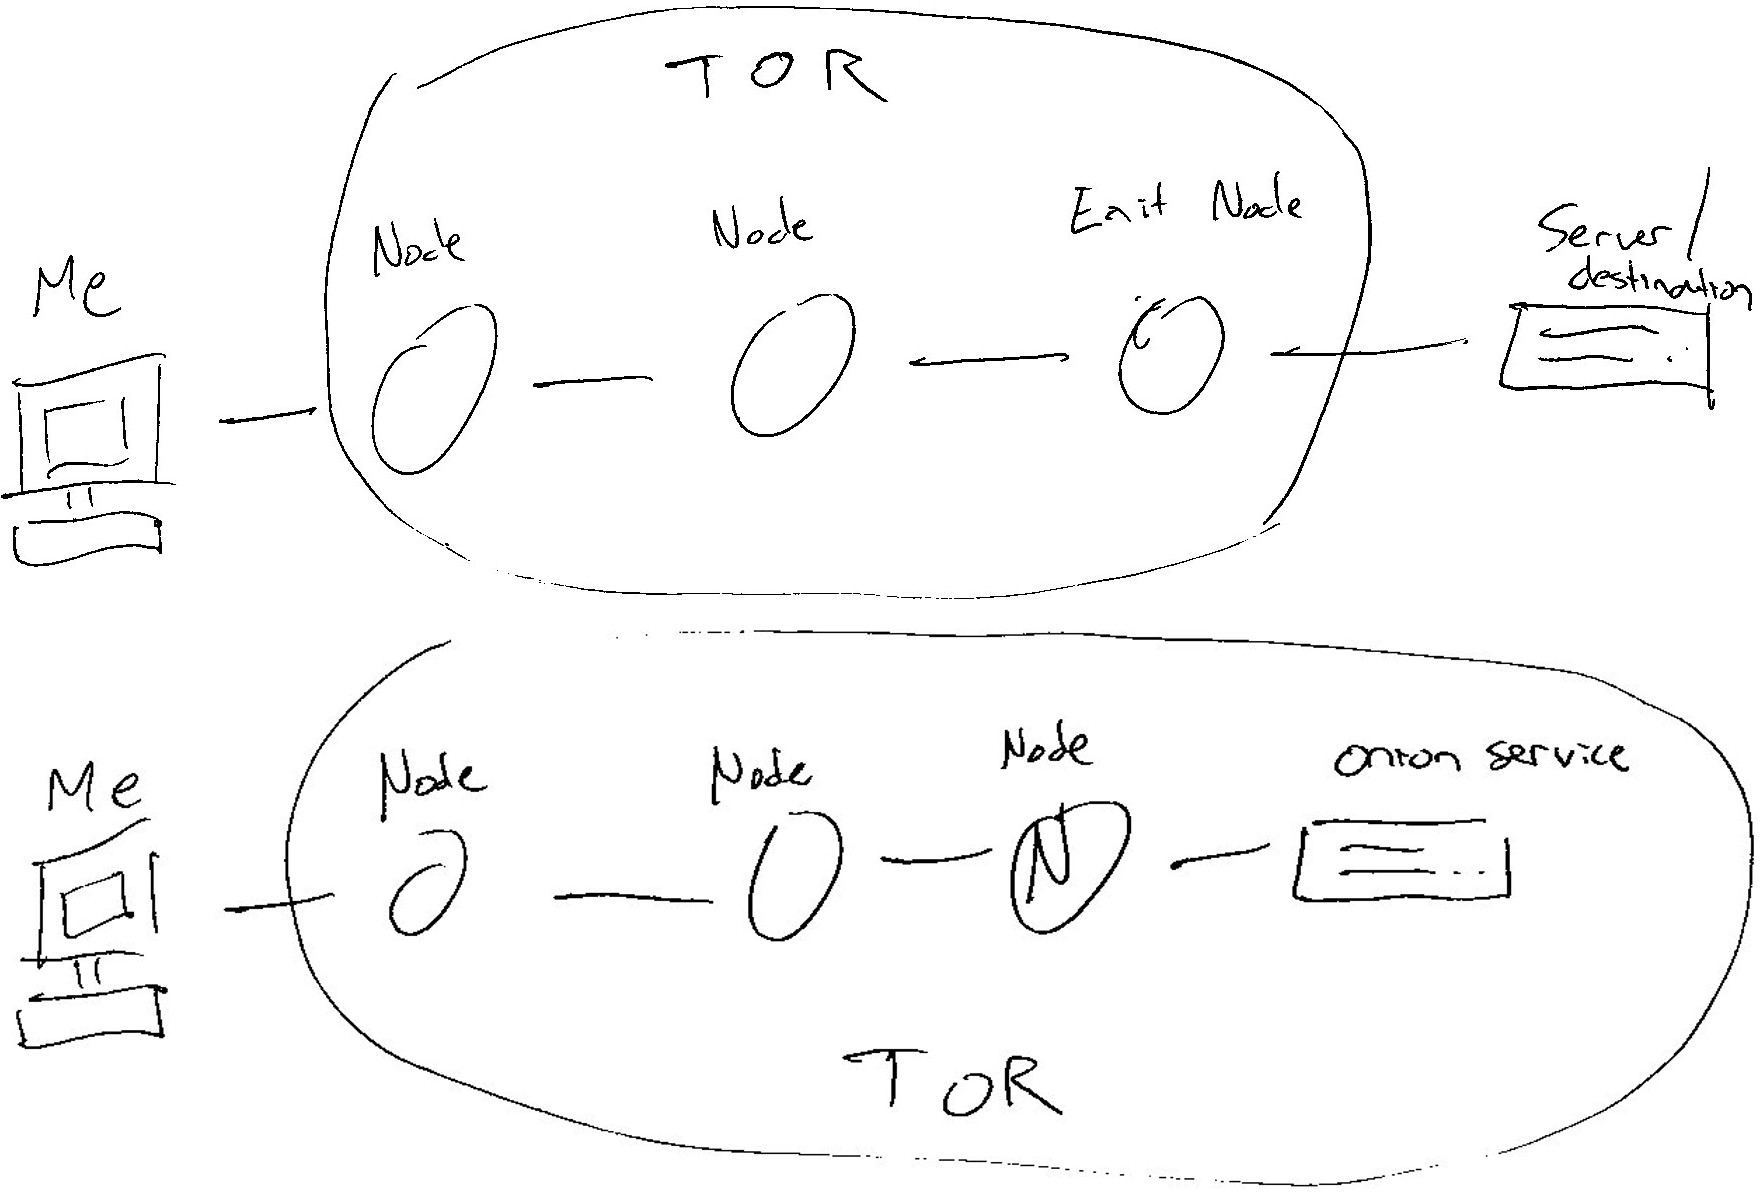
\includegraphics[width=0.8\linewidth]{figures/P13bothSketches.jpg}
        \caption{Comparison of two sketches of interviewee P13. First sketch shows the P13’s mental model of Tor and the second one P13’s mental model of Onion Services. }
        \label{fig:toros-sketch}
%    \caption{Sketches of two different,  interview participants of
%    how the onion services  work (top) and how onion services differ from Tor (bottom).}
\end{figure}




\subsubsection{The Puzzling Nature of Onion Services}
In our survey, we asked how safe our
respondents feel when using Tor Browser and onion services, respectively.
\Cref{fig:perceived-security} shows the results.  
86\% of our survey respondents feel at least somewhat safe using Tor Browser as compared to just over two thirds (67\%) of users of onion services.

\begin{figure}[t]
    \centering
    % Created by tikzDevice version 0.10.1 on 2018-01-12 16:35:49
% !TEX encoding = UTF-8 Unicode
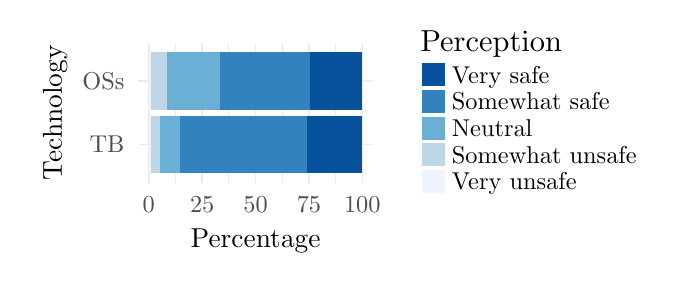
\begin{tikzpicture}[x=1pt,y=1pt]
\definecolor{fillColor}{RGB}{255,255,255}
\path[use as bounding box,fill=fillColor,fill opacity=0.00] (0,0) rectangle (231.26, 86.72);
\begin{scope}
\path[clip] ( 39.91, 30.77) rectangle (124.79, 81.22);
\definecolor{drawColor}{gray}{0.92}

\path[draw=drawColor,line width= 0.3pt,line join=round] ( 53.42, 30.77) --
	( 53.42, 81.22);

\path[draw=drawColor,line width= 0.3pt,line join=round] ( 72.71, 30.77) --
	( 72.71, 81.22);

\path[draw=drawColor,line width= 0.3pt,line join=round] ( 92.00, 30.77) --
	( 92.00, 81.22);

\path[draw=drawColor,line width= 0.3pt,line join=round] (111.29, 30.77) --
	(111.29, 81.22);

\path[draw=drawColor,line width= 0.6pt,line join=round] ( 39.91, 44.53) --
	(124.79, 44.53);

\path[draw=drawColor,line width= 0.6pt,line join=round] ( 39.91, 67.46) --
	(124.79, 67.46);

\path[draw=drawColor,line width= 0.6pt,line join=round] ( 43.77, 30.77) --
	( 43.77, 81.22);

\path[draw=drawColor,line width= 0.6pt,line join=round] ( 63.06, 30.77) --
	( 63.06, 81.22);

\path[draw=drawColor,line width= 0.6pt,line join=round] ( 82.35, 30.77) --
	( 82.35, 81.22);

\path[draw=drawColor,line width= 0.6pt,line join=round] (101.64, 30.77) --
	(101.64, 81.22);

\path[draw=drawColor,line width= 0.6pt,line join=round] (120.93, 30.77) --
	(120.93, 81.22);
\definecolor{fillColor}{RGB}{239,243,255}

\path[fill=fillColor] ( 43.77, 34.21) rectangle ( 44.51, 54.85);
\definecolor{fillColor}{RGB}{189,215,231}

\path[fill=fillColor] ( 44.51, 34.21) rectangle ( 47.92, 54.85);
\definecolor{fillColor}{RGB}{107,174,214}

\path[fill=fillColor] ( 47.92, 34.21) rectangle ( 54.90, 54.85);
\definecolor{fillColor}{RGB}{49,130,189}

\path[fill=fillColor] ( 54.90, 34.21) rectangle (100.90, 54.85);
\definecolor{fillColor}{RGB}{8,81,156}

\path[fill=fillColor] (100.90, 34.21) rectangle (120.93, 54.85);
\definecolor{fillColor}{RGB}{239,243,255}

\path[fill=fillColor] ( 43.77, 57.15) rectangle ( 44.67, 77.78);
\definecolor{fillColor}{RGB}{189,215,231}

\path[fill=fillColor] ( 44.67, 57.15) rectangle ( 50.19, 77.78);
\definecolor{fillColor}{RGB}{107,174,214}

\path[fill=fillColor] ( 50.19, 57.15) rectangle ( 69.60, 77.78);
\definecolor{fillColor}{RGB}{49,130,189}

\path[fill=fillColor] ( 69.60, 57.15) rectangle (101.98, 77.78);
\definecolor{fillColor}{RGB}{8,81,156}

\path[fill=fillColor] (101.98, 57.15) rectangle (120.93, 77.78);
\end{scope}
\begin{scope}
\path[clip] (  0.00,  0.00) rectangle (231.26, 86.72);
\definecolor{drawColor}{gray}{0.30}

\node[text=drawColor,anchor=base east,inner sep=0pt, outer sep=0pt, scale=  0.88] at ( 34.96, 41.50) {TB};

\node[text=drawColor,anchor=base east,inner sep=0pt, outer sep=0pt, scale=  0.88] at ( 34.96, 64.43) {OSs};
\end{scope}
\begin{scope}
\path[clip] (  0.00,  0.00) rectangle (231.26, 86.72);
\definecolor{drawColor}{gray}{0.30}

\node[text=drawColor,anchor=base,inner sep=0pt, outer sep=0pt, scale=  0.88] at ( 43.77, 19.76) {0};

\node[text=drawColor,anchor=base,inner sep=0pt, outer sep=0pt, scale=  0.88] at ( 63.06, 19.76) {25};

\node[text=drawColor,anchor=base,inner sep=0pt, outer sep=0pt, scale=  0.88] at ( 82.35, 19.76) {50};

\node[text=drawColor,anchor=base,inner sep=0pt, outer sep=0pt, scale=  0.88] at (101.64, 19.76) {75};

\node[text=drawColor,anchor=base,inner sep=0pt, outer sep=0pt, scale=  0.88] at (120.93, 19.76) {100};
\end{scope}
\begin{scope}
\path[clip] (  0.00,  0.00) rectangle (231.26, 86.72);
\definecolor{drawColor}{RGB}{0,0,0}

\node[text=drawColor,anchor=base,inner sep=0pt, outer sep=0pt, scale=  0.99] at ( 82.35,  7.44) {Percentage};
\end{scope}
\begin{scope}
\path[clip] (  0.00,  0.00) rectangle (231.26, 86.72);
\definecolor{drawColor}{RGB}{0,0,0}

\node[text=drawColor,rotate= 90.00,anchor=base,inner sep=0pt, outer sep=0pt, scale=  0.99] at ( 12.32, 56.00) {Technology};
\end{scope}
\begin{scope}
\path[clip] (  0.00,  0.00) rectangle (231.26, 86.72);
\definecolor{drawColor}{RGB}{0,0,0}

\node[text=drawColor,anchor=base west,inner sep=0pt, outer sep=0pt, scale=  1.10] at (141.86, 78.11) {Perception};
\end{scope}
\begin{scope}
\path[clip] (  0.00,  0.00) rectangle (231.26, 86.72);
\definecolor{fillColor}{RGB}{8,81,156}

\path[fill=fillColor] (142.58, 65.57) rectangle (150.79, 73.78);
\end{scope}
\begin{scope}
\path[clip] (  0.00,  0.00) rectangle (231.26, 86.72);
\definecolor{fillColor}{RGB}{49,130,189}

\path[fill=fillColor] (142.58, 55.93) rectangle (150.79, 64.15);
\end{scope}
\begin{scope}
\path[clip] (  0.00,  0.00) rectangle (231.26, 86.72);
\definecolor{fillColor}{RGB}{107,174,214}

\path[fill=fillColor] (142.58, 46.30) rectangle (150.79, 54.51);
\end{scope}
\begin{scope}
\path[clip] (  0.00,  0.00) rectangle (231.26, 86.72);
\definecolor{fillColor}{RGB}{189,215,231}

\path[fill=fillColor] (142.58, 36.66) rectangle (150.79, 44.87);
\end{scope}
\begin{scope}
\path[clip] (  0.00,  0.00) rectangle (231.26, 86.72);
\definecolor{fillColor}{RGB}{239,243,255}

\path[fill=fillColor] (142.58, 27.03) rectangle (150.79, 35.24);
\end{scope}
\begin{scope}
\path[clip] (  0.00,  0.00) rectangle (231.26, 86.72);
\definecolor{drawColor}{RGB}{0,0,0}

\node[text=drawColor,anchor=base west,inner sep=0pt, outer sep=0pt, scale=  0.88] at (153.31, 66.65) {Very safe};
\end{scope}
\begin{scope}
\path[clip] (  0.00,  0.00) rectangle (231.26, 86.72);
\definecolor{drawColor}{RGB}{0,0,0}

\node[text=drawColor,anchor=base west,inner sep=0pt, outer sep=0pt, scale=  0.88] at (153.31, 57.01) {Somewhat safe};
\end{scope}
\begin{scope}
\path[clip] (  0.00,  0.00) rectangle (231.26, 86.72);
\definecolor{drawColor}{RGB}{0,0,0}

\node[text=drawColor,anchor=base west,inner sep=0pt, outer sep=0pt, scale=  0.88] at (153.31, 47.37) {Neutral};
\end{scope}
\begin{scope}
\path[clip] (  0.00,  0.00) rectangle (231.26, 86.72);
\definecolor{drawColor}{RGB}{0,0,0}

\node[text=drawColor,anchor=base west,inner sep=0pt, outer sep=0pt, scale=  0.88] at (153.31, 37.74) {Somewhat unsafe};
\end{scope}
\begin{scope}
\path[clip] (  0.00,  0.00) rectangle (231.26, 86.72);
\definecolor{drawColor}{RGB}{0,0,0}

\node[text=drawColor,anchor=base west,inner sep=0pt, outer sep=0pt, scale=  0.88] at (153.31, 28.10) {Very unsafe};
\end{scope}
\end{tikzpicture}

    \caption{The level of safety our respondents perceive when using Tor
    Browser (\textsc{tb}) and onion services (\textsc{os}s).}
    \label{fig:perceived-security}
\end{figure}

Our survey responses indicated that our participants, many of whom were non-experts, \adz{how many?} lacked the ability to evaluate (or even understand) the
Tor network's design which is why they defer to expert opinion, their gut
feeling, or the trust they place in Tor developers.  With respect to onion
services, the majority of survey respondents expressed that the added security and anonymity makes
them feel safe.  Another factor contributing to the perceived security is that
advertising companies are nowhere near as present on onion services as they are
on the web.  Orthogonal to the technology, many participants voiced concern
about illegal and questionable content on onion services, described by some as a
``Wild West.'' Phishing sites, honeypots, and compromised onion sites further
contribute to this perception.

Although our interviewees tended to evaluate Onion links as safer than corresponding websites (8 vs. 4 participants), 6 people stressed that you need to be careful while using onion services. Five interviewees expressed lack of trust towards OS  and one even frustration.  Two interviewees mentioned that websites cannot identify you as the general advantage of onion services but one of these participants plus 2 others draw attention to the fact that websites actually can determine your identity if you write down your personal details as well as if you log in into any private accounts while using OS. Moreover, 1 interview participant (P10) claimed that using onion links may influence the usability of their ‘normal’ corresponding websites – he shared a story in which he postulated that his Facebook account had been flagged for suspicious activity and then was deactivated because he had logged in through Tor browser.  Nevertheless, P10 did not get any explanation from Facebook administrators. These interview participants did not realize that while the company indeed
knows who is logging in, it does not know Tor users' \textsc{ip} address (and
hence location) or operating system. On top of that, onion services provide
end-to-end security and self-authenticating names.  Syverson and Boyce took a
step back and looked at how onion services can improve website
authentication~\cite{Syverson2015a}.  These benefits are difficult to convey to
non-technical users, and even experts sometimes advocate an ``all or nothing''
approach to online anonymity, overlooking important nuances. 

Another source of confusion was the domain format of onion services.  Of all unique {\tt .onion} 
domains found in the root DNS data (22,966), about 33\% were an incorrect format; for example, 
\url{onion.onion} was found in the dataset, but is not a correctly formatted onion domain.

Additionally, some survey respondents commented on the onion domain format, indicating that they believed the seemingly-random
characters in onion domains are the reason why onion services are anonymous:

\begin{displayquote}[Survey respondent]
\ldots [The] Onion Services stay anonymous through changing their domain, and I
feel that there is a possibility of decreased anonymity with a constant domain
name.
\end{displayquote}

Accordingly, these users also believe that vanity domains are ``less anonymous''
because part of their domains is clearly not random.  A survey participant
further wrote: \textquote{I understand vanity onion domains are a sign of the
weakness of the hash algorithm used by the Tor network.}  An unrelated yet
equally incorrect opinion was voiced by a different survey respondent:
\textquote{These people who created their onion name using scallion or other
tools should notice that other people can make same private key.} Furthermoe, five interviewees expressed lack of trust towards OS like P06: “I'm pretty distrusting with most of the content I access over .onion services. When I want content from a service, I tend to distrust it from the beginning.” and one even frustration. On the other hand, 4 interviewees were content and believed in future of OS and 2 put trust in them.

What was perceived as another disadvantage by 4 of our interviewees was the fact that the URL strings of Onion links were considered long and among these participant was one who complained also on random numbers in URL strings. Two interviewees criticized onion links for being hard to remember. Moreover, \textsc{Url}s such as expyuzz4wqqyqhjn.onion and torproz4wqqyqhjn.onion were
harder for survey respondents to remember because they mention that ``numbers make the
names harder to remember.''  Other survey respondents stated that vanity domains are easier to
remember when they can be pronounced.  One survey respondent described it saying \mc{need participant id}
``phonetic pronunciation plays a large part in how I remember onions.'' Many
other survey \adz{how many} respondents stated that onion domains that are supported by a mnemonic are
also easier to remember.  
 

 One of the things that remain confusing is the terminology of OS; one interview participant named them as Dark Web, while another one as Hidden Services.  

 Another drawback of OS was identified in the latency and according to 3 participants the access time was too slow. 
 
\subsubsection{Versatility of Onion Services }
In the survey, we asked about how often our respondents browse onion
services.  The usage frequency was almost uniformly distributed among our survey
respondents; 24\% use onion sites less than once a month, 22\% use them about
monthly, 25\% weekly, and 23\% daily.  The remaining 6\% has never used an onion
service before.We also asked our interviewees whether they had used OS in the last 3 months and there was an equal division between those that answered: 7 had and 7 had not, with 4 of latter claiming that they had used it before, just not in the last 3 months and with 2 of them that had never used them before.

The majority of our survey participants  used onion services
because of the additional anonymity (70\%) and the additional security (61\%) (see \Cref{fig:onion-usage}). Moreover,  anonymity was also the main reason why interviewees used onion services (6/17). Another reassuring factor for two of our interviewees was sense of security and safety. Furthermore, two interview participants decided on onion services thinking of it as “harm reduction technique”, as P10 explained on Facebook example – he would rather use Facebook corresponding onion domain, in order to make his data harder to track, even though he did not believe it was a fully secure way to enter this site.

Moreover, 61.8\% of our survey respondents had used onion services for purposes
other than web browsing before.  Several protocols, such as the chat application
Ricochet~\cite{ricochet} and the file sharing application
OnionShare~\cite{onionshare}, were purpose-built on top of onion services while
existing \textsc{tcp}-based tools, such as \textsc{ssh}, can transparently use
onion addresses instead of traditional \textsc{ip} addresses.  Moreover, Pirate Bay (1), Ricochet (1), Tor Chat (1), Onion Share (1) as well as just Dark Web (1) were all mentioned by interviewees as reasons for using OS; our analysis of root DNS data corroborates this.  Some of the most common prefixes found in the data include cocaine, freedom, silkroad, alphabay, hosting, bitcoin, which are potentially representative of illicit (dark web) content. Almost one third
(29.7\%) of our survey participants used onion services for non-browsing activities at
least once a week. \mc{do we know what these were?}

Survey respondents who selected ``Other'' gave a variety of reasons, the most
predominant being the ability to set up a \textsc{tcp} service behind a
\textsc{nat} device.  That makes it possible to expose an \textsc{ssh} server in
a home network that has neither a permanent \textsc{ip} address nor port
forwarding.  Other survey respondents reported using onion services to reduce the load on exit relays, to do
technical research, and to access sites that are otherwise unavailable. There were also two interviewees that had an experience with OS only in an indirect way - One had not really browsed the OS by himself but had set up them for others, while another one used them not only for his work but also because it was his default set up.


There were also many task-oriented reasons that interview participants mentioned about. Almost one third (5) of interviewees reported that they use onion services simply for their work, while 4 – because of personal reasons, like personal blog or giving someone an access to his home network. Two interview participants used them for educational purposes but both in a different way - one (P03) as a teaching subject: “I was teaching a class on internet technology and regulations. We were basically showing students how Tor works and part of what I have to do as a teaching assistant was make students go and basically get to the moment where they either hire a hitman, buy drugs, or buy weapons. Just to show that it's possible. And then obviously we didn't buy it.” and another one (P05) for academic review process: “I've only used it for submitting academic papers. A lot of times we want to submit some source code, or some extra artifacts with it, but there's a problem if we host it on the university site. If one of the other reviewers connects to our university site, and we have some sort of tracking information on there, we would be deanonymizing the reviewer. We put it on a Tor hidden service to make sure that the reviewer remains blind in academic review process.” Moreover, one person reported that he uses onion services for his email account and one to communicate with others.

From a different perspective, for 46\% of the survey respondents and 3 interview respondents, it was the only way to access content they enjoy, making the use of
onion services a necessity. 27\% of our survey respondents and two interviewees admitted that they used it out of
curiosity. Moreover, 2 interview participants used OS for fun and social reasons – to “toy around” (P07) and also, as a way of spending time with friends, as well as to “show off” around them. 
 
Finally, 40\% of our survey respondents had once set up an onion service sometime in the past. 
Interestingly, 79\% of the survey respondents who had set up onion services of their own had run their onion service for
private use while 53\% had run them for the public. \Cref{fig:onion-operation-reasons} gives an overview of the reasons our
respondents have for running onion services. 


\begin{figure}[t]
    \centering
    % Created by tikzDevice version 0.10.1 on 2018-01-12 16:14:57
% !TEX encoding = UTF-8 Unicode
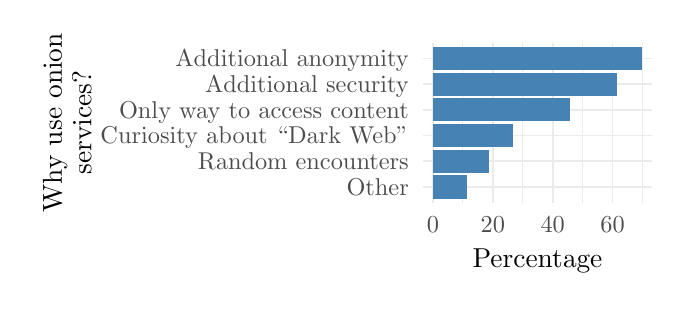
\begin{tikzpicture}[x=1pt,y=1pt]
\definecolor{fillColor}{RGB}{255,255,255}
\path[use as bounding box,fill=fillColor,fill opacity=0.00] (0,0) rectangle (231.26, 93.95);
\begin{scope}
\path[clip] (142.68, 30.77) rectangle (225.76, 88.45);
\definecolor{drawColor}{gray}{0.92}

\path[draw=drawColor,line width= 0.3pt,line join=round] (157.27, 30.77) --
	(157.27, 88.45);

\path[draw=drawColor,line width= 0.3pt,line join=round] (178.90, 30.77) --
	(178.90, 88.45);

\path[draw=drawColor,line width= 0.3pt,line join=round] (200.54, 30.77) --
	(200.54, 88.45);

\path[draw=drawColor,line width= 0.3pt,line join=round] (222.17, 30.77) --
	(222.17, 88.45);

\path[draw=drawColor,line width= 0.6pt,line join=round] (142.68, 36.35) --
	(225.76, 36.35);

\path[draw=drawColor,line width= 0.6pt,line join=round] (142.68, 45.66) --
	(225.76, 45.66);

\path[draw=drawColor,line width= 0.6pt,line join=round] (142.68, 54.96) --
	(225.76, 54.96);

\path[draw=drawColor,line width= 0.6pt,line join=round] (142.68, 64.26) --
	(225.76, 64.26);

\path[draw=drawColor,line width= 0.6pt,line join=round] (142.68, 73.57) --
	(225.76, 73.57);

\path[draw=drawColor,line width= 0.6pt,line join=round] (142.68, 82.87) --
	(225.76, 82.87);

\path[draw=drawColor,line width= 0.6pt,line join=round] (146.45, 30.77) --
	(146.45, 88.45);

\path[draw=drawColor,line width= 0.6pt,line join=round] (168.09, 30.77) --
	(168.09, 88.45);

\path[draw=drawColor,line width= 0.6pt,line join=round] (189.72, 30.77) --
	(189.72, 88.45);

\path[draw=drawColor,line width= 0.6pt,line join=round] (211.35, 30.77) --
	(211.35, 88.45);
\definecolor{fillColor}{RGB}{70,130,180}

\path[fill=fillColor] (146.45, 32.17) rectangle (158.77, 40.54);

\path[fill=fillColor] (146.45, 41.47) rectangle (166.57, 49.84);

\path[fill=fillColor] (146.45, 50.77) rectangle (175.40, 59.15);

\path[fill=fillColor] (146.45, 60.08) rectangle (196.12, 68.45);

\path[fill=fillColor] (146.45, 69.38) rectangle (212.96, 77.75);

\path[fill=fillColor] (146.45, 78.68) rectangle (221.99, 87.06);
\end{scope}
\begin{scope}
\path[clip] (  0.00,  0.00) rectangle (231.26, 93.95);
\definecolor{drawColor}{gray}{0.30}

\node[text=drawColor,anchor=base east,inner sep=0pt, outer sep=0pt, scale=  0.88] at (137.73, 33.32) {Other};

\node[text=drawColor,anchor=base east,inner sep=0pt, outer sep=0pt, scale=  0.88] at (137.73, 42.63) {Random encounters};

\node[text=drawColor,anchor=base east,inner sep=0pt, outer sep=0pt, scale=  0.88] at (137.73, 51.93) {Curiosity about ``Dark Web''};

\node[text=drawColor,anchor=base east,inner sep=0pt, outer sep=0pt, scale=  0.88] at (137.73, 61.23) {Only way to access content};

\node[text=drawColor,anchor=base east,inner sep=0pt, outer sep=0pt, scale=  0.88] at (137.73, 70.54) {Additional security};

\node[text=drawColor,anchor=base east,inner sep=0pt, outer sep=0pt, scale=  0.88] at (137.73, 79.84) {Additional anonymity};
\end{scope}
\begin{scope}
\path[clip] (  0.00,  0.00) rectangle (231.26, 93.95);
\definecolor{drawColor}{gray}{0.30}

\node[text=drawColor,anchor=base,inner sep=0pt, outer sep=0pt, scale=  0.88] at (146.45, 19.76) {0};

\node[text=drawColor,anchor=base,inner sep=0pt, outer sep=0pt, scale=  0.88] at (168.09, 19.76) {20};

\node[text=drawColor,anchor=base,inner sep=0pt, outer sep=0pt, scale=  0.88] at (189.72, 19.76) {40};

\node[text=drawColor,anchor=base,inner sep=0pt, outer sep=0pt, scale=  0.88] at (211.35, 19.76) {60};
\end{scope}
\begin{scope}
\path[clip] (  0.00,  0.00) rectangle (231.26, 93.95);
\definecolor{drawColor}{RGB}{0,0,0}

\node[text=drawColor,anchor=base,inner sep=0pt, outer sep=0pt, scale=  0.99] at (184.22,  7.44) {Percentage};
\end{scope}
\begin{scope}
\path[clip] (  0.00,  0.00) rectangle (231.26, 93.95);
\definecolor{drawColor}{RGB}{0,0,0}

\node[text=drawColor,rotate= 90.00,anchor=base,inner sep=0pt, outer sep=0pt, scale=  0.99] at ( 12.32, 59.61) {Why use onion};

\node[text=drawColor,rotate= 90.00,anchor=base,inner sep=0pt, outer sep=0pt, scale=  0.99] at ( 23.01, 59.61) {services?};
\end{scope}
\end{tikzpicture}

    \caption{Our respondents' (multiple choice) reasons for using onion
    services.}
    \label{fig:onion-usage}
\end{figure}



\begin{figure}[t]
    \centering
    % Created by tikzDevice version 0.10.1 on 2018-01-12 16:24:46
% !TEX encoding = UTF-8 Unicode
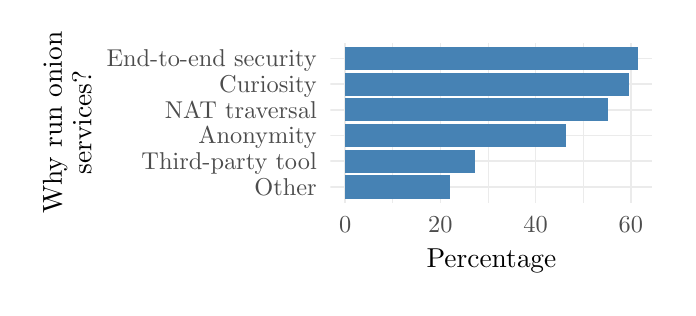
\begin{tikzpicture}[x=1pt,y=1pt]
\definecolor{fillColor}{RGB}{255,255,255}
\path[use as bounding box,fill=fillColor,fill opacity=0.00] (0,0) rectangle (231.26, 93.95);
\begin{scope}
\path[clip] (109.42, 30.77) rectangle (225.76, 88.45);
\definecolor{drawColor}{gray}{0.92}

\path[draw=drawColor,line width= 0.3pt,line join=round] (131.91, 30.77) --
	(131.91, 88.45);

\path[draw=drawColor,line width= 0.3pt,line join=round] (166.33, 30.77) --
	(166.33, 88.45);

\path[draw=drawColor,line width= 0.3pt,line join=round] (200.75, 30.77) --
	(200.75, 88.45);

\path[draw=drawColor,line width= 0.6pt,line join=round] (109.42, 36.35) --
	(225.76, 36.35);

\path[draw=drawColor,line width= 0.6pt,line join=round] (109.42, 45.66) --
	(225.76, 45.66);

\path[draw=drawColor,line width= 0.6pt,line join=round] (109.42, 54.96) --
	(225.76, 54.96);

\path[draw=drawColor,line width= 0.6pt,line join=round] (109.42, 64.26) --
	(225.76, 64.26);

\path[draw=drawColor,line width= 0.6pt,line join=round] (109.42, 73.57) --
	(225.76, 73.57);

\path[draw=drawColor,line width= 0.6pt,line join=round] (109.42, 82.87) --
	(225.76, 82.87);

\path[draw=drawColor,line width= 0.6pt,line join=round] (114.70, 30.77) --
	(114.70, 88.45);

\path[draw=drawColor,line width= 0.6pt,line join=round] (149.12, 30.77) --
	(149.12, 88.45);

\path[draw=drawColor,line width= 0.6pt,line join=round] (183.54, 30.77) --
	(183.54, 88.45);

\path[draw=drawColor,line width= 0.6pt,line join=round] (217.96, 30.77) --
	(217.96, 88.45);
\definecolor{fillColor}{RGB}{70,130,180}

\path[fill=fillColor] (114.70, 32.17) rectangle (152.48, 40.54);

\path[fill=fillColor] (114.70, 41.47) rectangle (161.72, 49.84);

\path[fill=fillColor] (114.70, 50.77) rectangle (194.45, 59.15);

\path[fill=fillColor] (114.70, 60.08) rectangle (209.56, 68.45);

\path[fill=fillColor] (114.70, 69.38) rectangle (217.12, 77.75);

\path[fill=fillColor] (114.70, 78.68) rectangle (220.48, 87.06);
\end{scope}
\begin{scope}
\path[clip] (  0.00,  0.00) rectangle (231.26, 93.95);
\definecolor{drawColor}{gray}{0.30}

\node[text=drawColor,anchor=base east,inner sep=0pt, outer sep=0pt, scale=  0.88] at (104.47, 33.32) {Other};

\node[text=drawColor,anchor=base east,inner sep=0pt, outer sep=0pt, scale=  0.88] at (104.47, 42.63) {Third-party tool};

\node[text=drawColor,anchor=base east,inner sep=0pt, outer sep=0pt, scale=  0.88] at (104.47, 51.93) {Anonymity};

\node[text=drawColor,anchor=base east,inner sep=0pt, outer sep=0pt, scale=  0.88] at (104.47, 61.23) {NAT traversal};

\node[text=drawColor,anchor=base east,inner sep=0pt, outer sep=0pt, scale=  0.88] at (104.47, 70.54) {Curiosity};

\node[text=drawColor,anchor=base east,inner sep=0pt, outer sep=0pt, scale=  0.88] at (104.47, 79.84) {End-to-end security};
\end{scope}
\begin{scope}
\path[clip] (  0.00,  0.00) rectangle (231.26, 93.95);
\definecolor{drawColor}{gray}{0.30}

\node[text=drawColor,anchor=base,inner sep=0pt, outer sep=0pt, scale=  0.88] at (114.70, 19.76) {0};

\node[text=drawColor,anchor=base,inner sep=0pt, outer sep=0pt, scale=  0.88] at (149.12, 19.76) {20};

\node[text=drawColor,anchor=base,inner sep=0pt, outer sep=0pt, scale=  0.88] at (183.54, 19.76) {40};

\node[text=drawColor,anchor=base,inner sep=0pt, outer sep=0pt, scale=  0.88] at (217.96, 19.76) {60};
\end{scope}
\begin{scope}
\path[clip] (  0.00,  0.00) rectangle (231.26, 93.95);
\definecolor{drawColor}{RGB}{0,0,0}

\node[text=drawColor,anchor=base,inner sep=0pt, outer sep=0pt, scale=  0.99] at (167.59,  7.44) {Percentage};
\end{scope}
\begin{scope}
\path[clip] (  0.00,  0.00) rectangle (231.26, 93.95);
\definecolor{drawColor}{RGB}{0,0,0}

\node[text=drawColor,rotate= 90.00,anchor=base,inner sep=0pt, outer sep=0pt, scale=  0.99] at ( 12.32, 59.61) {Why run onion};

\node[text=drawColor,rotate= 90.00,anchor=base,inner sep=0pt, outer sep=0pt, scale=  0.99] at ( 23.01, 59.61) {services?};
\end{scope}
\end{tikzpicture}

    \caption{The (multiple-choice) reasons our respondents have for running
    onion services.}
    \label{fig:onion-operation-reasons}
\end{figure}

\subsection{Onion Service Discovery \& Management}
\label{sec:manage}

\subsubsection{Onion Links Usually Discovered on Social Media, on the Web, Via Search Engines But Also By Chance}
Recall that a freshly set up onion service is private by default, leaving it up
to its operator to disseminate the domain.  Established search engines such as
Google are therefore inadequate to find content on onion services.  We wanted to
find out how our participants discover onion services.
\Cref{fig:onion-discovery} illustrates the results of our survey.  The three most popular ways
that survey participants discovered new onion sites, all approximating 50\%, were via \first~social
networking sites such as Twitter and Reddit, \second~the list of search engines
such as Ahmia,\footnote{Ahmia.fi is an onion site search engine that crawls
user-submitted onion domains.  It publishes the list of all indexed onion
services at \url{https://ahmia.fi/onions/}.} and \third~randomly encountering
links when browsing the web. 
We observed very similar pattern in our interview respondents – almost the same 3 leading ways of searching for new onion links.  We categorized them in word of mouth (6), using a search engine tool (5) including tools like duckduckgo (1), .go (1), Pirate Bay (1), Reddit (1), .fiahima (1), onion wictionary (2) and search widget in the Tor browser (1). Moreover, 6 of our participants were more likely to look for onion services passively, so they just happened to hear or know about specific onion link, while five of them looked actively for onion links, browsing for the content they needed.

While significantly less popular method among our survey participants for discovering onion domains was through friends and
family, which had the advantage that domains come from a trusted source. \adz{how many?}
Finally, 19\% of survey respondents occasionally
stumbled upon links to onion services in their day-to-day browsing activity, while
a mere
4\% of our survey respondents indicated that they were not interested in learning about new onion services and two interviewees claimed that they never searched for new Onion links.
Respondents who selected ``Other'' predominantly brought up
independently-maintained onion domain aggregators.  A noteworthy example is the
Hidden Wiki, a community-curated and frequently-forked wiki that contains
categorized links to onion services.  As a further matter, two interview participants reported they would look up for them also through public Internet and two would find them via other onion websites.

\begin{figure}[t]
    \centering
    % Created by tikzDevice version 0.10.1 on 2018-01-12 16:15:03
% !TEX encoding = UTF-8 Unicode
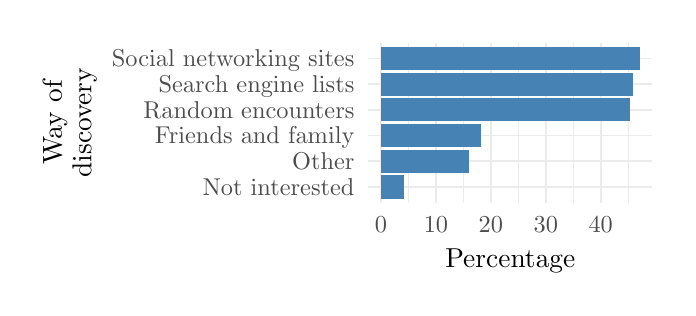
\begin{tikzpicture}[x=1pt,y=1pt]
\definecolor{fillColor}{RGB}{255,255,255}
\path[use as bounding box,fill=fillColor,fill opacity=0.00] (0,0) rectangle (231.26, 93.95);
\begin{scope}
\path[clip] (123.02, 30.77) rectangle (225.76, 88.45);
\definecolor{drawColor}{gray}{0.92}

\path[draw=drawColor,line width= 0.3pt,line join=round] (137.61, 30.77) --
	(137.61, 88.45);

\path[draw=drawColor,line width= 0.3pt,line join=round] (157.46, 30.77) --
	(157.46, 88.45);

\path[draw=drawColor,line width= 0.3pt,line join=round] (177.31, 30.77) --
	(177.31, 88.45);

\path[draw=drawColor,line width= 0.3pt,line join=round] (197.16, 30.77) --
	(197.16, 88.45);

\path[draw=drawColor,line width= 0.3pt,line join=round] (217.00, 30.77) --
	(217.00, 88.45);

\path[draw=drawColor,line width= 0.6pt,line join=round] (123.02, 36.35) --
	(225.76, 36.35);

\path[draw=drawColor,line width= 0.6pt,line join=round] (123.02, 45.66) --
	(225.76, 45.66);

\path[draw=drawColor,line width= 0.6pt,line join=round] (123.02, 54.96) --
	(225.76, 54.96);

\path[draw=drawColor,line width= 0.6pt,line join=round] (123.02, 64.26) --
	(225.76, 64.26);

\path[draw=drawColor,line width= 0.6pt,line join=round] (123.02, 73.57) --
	(225.76, 73.57);

\path[draw=drawColor,line width= 0.6pt,line join=round] (123.02, 82.87) --
	(225.76, 82.87);

\path[draw=drawColor,line width= 0.6pt,line join=round] (127.69, 30.77) --
	(127.69, 88.45);

\path[draw=drawColor,line width= 0.6pt,line join=round] (147.54, 30.77) --
	(147.54, 88.45);

\path[draw=drawColor,line width= 0.6pt,line join=round] (167.38, 30.77) --
	(167.38, 88.45);

\path[draw=drawColor,line width= 0.6pt,line join=round] (187.23, 30.77) --
	(187.23, 88.45);

\path[draw=drawColor,line width= 0.6pt,line join=round] (207.08, 30.77) --
	(207.08, 88.45);
\definecolor{fillColor}{RGB}{70,130,180}

\path[fill=fillColor] (127.69, 32.17) rectangle (135.96, 40.54);

\path[fill=fillColor] (127.69, 41.47) rectangle (159.33, 49.84);

\path[fill=fillColor] (127.69, 50.77) rectangle (163.85, 59.15);

\path[fill=fillColor] (127.69, 60.08) rectangle (217.70, 68.45);

\path[fill=fillColor] (127.69, 69.38) rectangle (218.83, 77.75);

\path[fill=fillColor] (127.69, 78.68) rectangle (221.09, 87.06);
\end{scope}
\begin{scope}
\path[clip] (  0.00,  0.00) rectangle (231.26, 93.95);
\definecolor{drawColor}{gray}{0.30}

\node[text=drawColor,anchor=base east,inner sep=0pt, outer sep=0pt, scale=  0.88] at (118.07, 33.32) {Not interested};

\node[text=drawColor,anchor=base east,inner sep=0pt, outer sep=0pt, scale=  0.88] at (118.07, 42.63) {Other};

\node[text=drawColor,anchor=base east,inner sep=0pt, outer sep=0pt, scale=  0.88] at (118.07, 51.93) {Friends and family};

\node[text=drawColor,anchor=base east,inner sep=0pt, outer sep=0pt, scale=  0.88] at (118.07, 61.23) {Random encounters};

\node[text=drawColor,anchor=base east,inner sep=0pt, outer sep=0pt, scale=  0.88] at (118.07, 70.54) {Search engine lists};

\node[text=drawColor,anchor=base east,inner sep=0pt, outer sep=0pt, scale=  0.88] at (118.07, 79.84) {Social networking sites};
\end{scope}
\begin{scope}
\path[clip] (  0.00,  0.00) rectangle (231.26, 93.95);
\definecolor{drawColor}{gray}{0.30}

\node[text=drawColor,anchor=base,inner sep=0pt, outer sep=0pt, scale=  0.88] at (127.69, 19.76) {0};

\node[text=drawColor,anchor=base,inner sep=0pt, outer sep=0pt, scale=  0.88] at (147.54, 19.76) {10};

\node[text=drawColor,anchor=base,inner sep=0pt, outer sep=0pt, scale=  0.88] at (167.38, 19.76) {20};

\node[text=drawColor,anchor=base,inner sep=0pt, outer sep=0pt, scale=  0.88] at (187.23, 19.76) {30};

\node[text=drawColor,anchor=base,inner sep=0pt, outer sep=0pt, scale=  0.88] at (207.08, 19.76) {40};
\end{scope}
\begin{scope}
\path[clip] (  0.00,  0.00) rectangle (231.26, 93.95);
\definecolor{drawColor}{RGB}{0,0,0}

\node[text=drawColor,anchor=base,inner sep=0pt, outer sep=0pt, scale=  0.99] at (174.39,  7.44) {Percentage};
\end{scope}
\begin{scope}
\path[clip] (  0.00,  0.00) rectangle (231.26, 93.95);
\definecolor{drawColor}{RGB}{0,0,0}

\node[text=drawColor,rotate= 90.00,anchor=base,inner sep=0pt, outer sep=0pt, scale=  0.99] at ( 12.32, 59.61) {Way of};

\node[text=drawColor,rotate= 90.00,anchor=base,inner sep=0pt, outer sep=0pt, scale=  0.99] at ( 23.01, 59.61) {discovery};
\end{scope}
\end{tikzpicture}

    \caption{Our respondents' (multiple choice) methods of discovering onion
    services.}
    \label{fig:onion-discovery}
\end{figure}

The majority of our survey respondents (60\%) reported that they were satisfied with how they discover onion services but a significant proportion (40\%) were not. Those who were satisfied with how they discover onion links reported that they have no
interest in learning about new onion services, in part because they only use a
small set of onion services.  



\begin{figure}[t]
    \centering
    % Created by tikzDevice version 0.10.1 on 2018-02-09 14:36:33
% !TEX encoding = UTF-8 Unicode
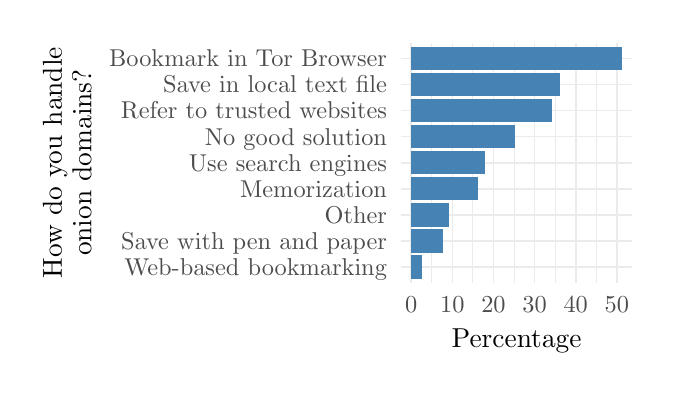
\begin{tikzpicture}[x=1pt,y=1pt]
\definecolor{fillColor}{RGB}{255,255,255}
\path[use as bounding box,fill=fillColor,fill opacity=0.00] (0,0) rectangle (224.04,122.86);
\begin{scope}
\path[clip] (134.78, 30.77) rectangle (218.54,117.36);
\definecolor{drawColor}{gray}{0.92}

\path[draw=drawColor,line width= 0.3pt,line join=round] (146.02, 30.77) --
	(146.02,117.36);

\path[draw=drawColor,line width= 0.3pt,line join=round] (160.88, 30.77) --
	(160.88,117.36);

\path[draw=drawColor,line width= 0.3pt,line join=round] (175.74, 30.77) --
	(175.74,117.36);

\path[draw=drawColor,line width= 0.3pt,line join=round] (190.61, 30.77) --
	(190.61,117.36);

\path[draw=drawColor,line width= 0.3pt,line join=round] (205.47, 30.77) --
	(205.47,117.36);

\path[draw=drawColor,line width= 0.6pt,line join=round] (134.78, 36.42) --
	(218.54, 36.42);

\path[draw=drawColor,line width= 0.6pt,line join=round] (134.78, 45.83) --
	(218.54, 45.83);

\path[draw=drawColor,line width= 0.6pt,line join=round] (134.78, 55.24) --
	(218.54, 55.24);

\path[draw=drawColor,line width= 0.6pt,line join=round] (134.78, 64.65) --
	(218.54, 64.65);

\path[draw=drawColor,line width= 0.6pt,line join=round] (134.78, 74.07) --
	(218.54, 74.07);

\path[draw=drawColor,line width= 0.6pt,line join=round] (134.78, 83.48) --
	(218.54, 83.48);

\path[draw=drawColor,line width= 0.6pt,line join=round] (134.78, 92.89) --
	(218.54, 92.89);

\path[draw=drawColor,line width= 0.6pt,line join=round] (134.78,102.30) --
	(218.54,102.30);

\path[draw=drawColor,line width= 0.6pt,line join=round] (134.78,111.71) --
	(218.54,111.71);

\path[draw=drawColor,line width= 0.6pt,line join=round] (138.58, 30.77) --
	(138.58,117.36);

\path[draw=drawColor,line width= 0.6pt,line join=round] (153.45, 30.77) --
	(153.45,117.36);

\path[draw=drawColor,line width= 0.6pt,line join=round] (168.31, 30.77) --
	(168.31,117.36);

\path[draw=drawColor,line width= 0.6pt,line join=round] (183.17, 30.77) --
	(183.17,117.36);

\path[draw=drawColor,line width= 0.6pt,line join=round] (198.04, 30.77) --
	(198.04,117.36);

\path[draw=drawColor,line width= 0.6pt,line join=round] (212.90, 30.77) --
	(212.90,117.36);
\definecolor{fillColor}{RGB}{70,130,180}

\path[fill=fillColor] (138.58, 32.18) rectangle (142.54, 40.66);

\path[fill=fillColor] (138.58, 41.60) rectangle (150.15, 50.07);

\path[fill=fillColor] (138.58, 51.01) rectangle (152.13, 59.48);

\path[fill=fillColor] (138.58, 60.42) rectangle (162.84, 68.89);

\path[fill=fillColor] (138.58, 69.83) rectangle (165.10, 78.30);

\path[fill=fillColor] (138.58, 79.24) rectangle (176.10, 87.71);

\path[fill=fillColor] (138.58, 88.65) rectangle (189.36, 97.12);

\path[fill=fillColor] (138.58, 98.07) rectangle (192.45,106.54);

\path[fill=fillColor] (138.58,107.48) rectangle (214.73,115.95);
\end{scope}
\begin{scope}
\path[clip] (  0.00,  0.00) rectangle (224.04,122.86);
\definecolor{drawColor}{gray}{0.30}

\node[text=drawColor,anchor=base east,inner sep=0pt, outer sep=0pt, scale=  0.88] at (129.83, 33.39) {Web-based bookmarking};

\node[text=drawColor,anchor=base east,inner sep=0pt, outer sep=0pt, scale=  0.88] at (129.83, 42.80) {Save with pen and paper};

\node[text=drawColor,anchor=base east,inner sep=0pt, outer sep=0pt, scale=  0.88] at (129.83, 52.21) {Other};

\node[text=drawColor,anchor=base east,inner sep=0pt, outer sep=0pt, scale=  0.88] at (129.83, 61.62) {Memorization};

\node[text=drawColor,anchor=base east,inner sep=0pt, outer sep=0pt, scale=  0.88] at (129.83, 71.04) {Use search engines};

\node[text=drawColor,anchor=base east,inner sep=0pt, outer sep=0pt, scale=  0.88] at (129.83, 80.45) {No good solution};

\node[text=drawColor,anchor=base east,inner sep=0pt, outer sep=0pt, scale=  0.88] at (129.83, 89.86) {Refer to trusted websites};

\node[text=drawColor,anchor=base east,inner sep=0pt, outer sep=0pt, scale=  0.88] at (129.83, 99.27) {Save in local text file};

\node[text=drawColor,anchor=base east,inner sep=0pt, outer sep=0pt, scale=  0.88] at (129.83,108.68) {Bookmark in Tor Browser};
\end{scope}
\begin{scope}
\path[clip] (  0.00,  0.00) rectangle (224.04,122.86);
\definecolor{drawColor}{gray}{0.30}

\node[text=drawColor,anchor=base,inner sep=0pt, outer sep=0pt, scale=  0.88] at (138.58, 19.76) {0};

\node[text=drawColor,anchor=base,inner sep=0pt, outer sep=0pt, scale=  0.88] at (153.45, 19.76) {10};

\node[text=drawColor,anchor=base,inner sep=0pt, outer sep=0pt, scale=  0.88] at (168.31, 19.76) {20};

\node[text=drawColor,anchor=base,inner sep=0pt, outer sep=0pt, scale=  0.88] at (183.17, 19.76) {30};

\node[text=drawColor,anchor=base,inner sep=0pt, outer sep=0pt, scale=  0.88] at (198.04, 19.76) {40};

\node[text=drawColor,anchor=base,inner sep=0pt, outer sep=0pt, scale=  0.88] at (212.90, 19.76) {50};
\end{scope}
\begin{scope}
\path[clip] (  0.00,  0.00) rectangle (224.04,122.86);
\definecolor{drawColor}{RGB}{0,0,0}

\node[text=drawColor,anchor=base,inner sep=0pt, outer sep=0pt, scale=  0.99] at (176.66,  7.44) {Percentage};
\end{scope}
\begin{scope}
\path[clip] (  0.00,  0.00) rectangle (224.04,122.86);
\definecolor{drawColor}{RGB}{0,0,0}

\node[text=drawColor,rotate= 90.00,anchor=base,inner sep=0pt, outer sep=0pt, scale=  0.99] at ( 12.32, 74.07) {How do you handle};

\node[text=drawColor,rotate= 90.00,anchor=base,inner sep=0pt, outer sep=0pt, scale=  0.99] at ( 23.01, 74.07) {onion domains?};
\end{scope}
\end{tikzpicture}

    \caption{The strategies that our respondents use to handle onion domains.
    More than half use bookmarks inside of Tor Browser and a quarter thinks that
    there is no good solution.}
    \label{fig:onion-domain-mgmt}
\end{figure}


\subsubsection{Saving and Tracking Onion Links Is Not Straightforward}
While conventional domains are designed to be easy to remember and recognize, we wanted to know how users handle randomly-generated onion domains. Most survey respondents use Tor Browser's bookmarks to save onion domains as seen in \Cref{fig:onion-domain-mgmt}. Additionally, same tactic used two interview participants.   While
convenient, this method of saving onion links leaves a trace of (presumably) visited sites on somebody's
computer.  One of Tor Browser's security requirements is ``disk avoidance,''
\ie, the browser must not write anything to disk that would reveal the user's
browsing history~\cite[\S~2.1]{Perry2017a}.  Bookmarking links is a violation of
this security requirement albeit requested by the user.  Many of our survey respondents
were aware of this issue, and about a dozen survey respondents who selected ``Other'' stated that they store onion domains in an encrypted manner---either in a text file or in their password manager.  Somewhat less popular amongst our survey participants was saving onion domains in local text files (36\%), getting them from trusted web sites (34\%), using search engines (18\%), memorizing domains (16\%), using some other 
techniques (9\%), or employing pen and paper (8\%).  When it comes to our interviewees, it seemed that they liked the old fashioned way the most for keeping track on onion links  - 4 reported that they keep them simply as a list and a note, furthermore 3 use their memory as storage place, simply remembering the addresses. Apart from these, one interviewee used his Twitter feed and another Tor chat as storage places. Moreover one interviewee stated that Tor browser remembers the links and another interview participant (P01) explained: “The onion services we run professionally we keep track of because we operate the server, so that's easy”. Notably, one quarter of our survey
respondents did not have a good solution to the problem of tracking onion links and  two interviewees admitted that they did not have any storage system for Onion links.
Given the alarming
number of (possibly insecure) home-baked solutions, a Tor Browser extension that
solves this problem seems warranted.

Of the survey respondents who memorize onion domains, we found that most respondents
memorize one to four onion domains (35\% of total respondents) but only 1\% are able to memorize more than four domains.   Survey respondents memorized domains \first~automatically start to memorize domains
because of typing it many times (60\%)
\second~to allow them to open the site more
quickly (51\%), and \third~to ensure that they are visiting the correct site and
not a phishing site (44\%). Others were privacy conscious because as mentioned above,
bookmarking onion domains leaves a trace. These 28\% of survey respondents said
they memorized onion domains to prevent this digital trace.

The majority of our survey respondents appreciated vanity domains because they were easy
to remember (64\%) and easy to recognize (64\%), and they provided a unique
``branding'' (34\%).  Some survey respondents indicated that a vanity prefix---like a
traditional domain---informs about an onion service's content, letting visitors
know what to expect and thus preventing unpleasant surprises.  Only 8\% disliked
vanity onion domains, and 15\% did not have an opinion.  We asked survey respondents
about whether or not they memorize vanity domains---specifically
facebookcorewwwi.onion---and how difficult they find it to memorize onion
domains of differing levels of vanity.  59\% of respondents replied that
facebookcorewwwi.onion is among the sites that they have memorized.  This is \mc{what are the participant or survey respondent ids for the quotes}
because it is ``easy to memorize'' and ``after seeing [it] many times, I
automatically start to memorize it.'' Depending on the format of the vanity domain, our survey respondents expressed differing levels of ease for
memorizing them; these results are shown in \Cref{fig:memorize-domains}.

\begin{figure}[t]
    \centering
    % Created by tikzDevice version 0.10.1 on 2018-02-09 14:43:10
% !TEX encoding = UTF-8 Unicode
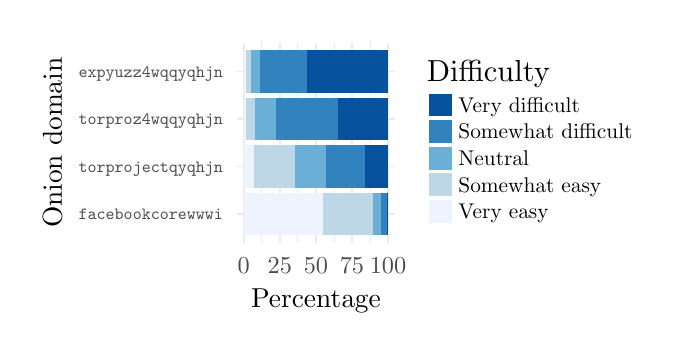
\begin{tikzpicture}[x=1pt,y=1pt]
\definecolor{fillColor}{RGB}{255,255,255}
\path[use as bounding box,fill=fillColor,fill opacity=0.00] (0,0) rectangle (224.04,108.41);
\begin{scope}
\path[clip] ( 75.47, 30.77) rectangle (132.84,102.91);
\definecolor{drawColor}{gray}{0.92}

\path[draw=drawColor,line width= 0.3pt,line join=round] ( 84.60, 30.77) --
	( 84.60,102.91);

\path[draw=drawColor,line width= 0.3pt,line join=round] ( 97.64, 30.77) --
	( 97.64,102.91);

\path[draw=drawColor,line width= 0.3pt,line join=round] (110.67, 30.77) --
	(110.67,102.91);

\path[draw=drawColor,line width= 0.3pt,line join=round] (123.71, 30.77) --
	(123.71,102.91);

\path[draw=drawColor,line width= 0.6pt,line join=round] ( 75.47, 41.08) --
	(132.84, 41.08);

\path[draw=drawColor,line width= 0.6pt,line join=round] ( 75.47, 58.25) --
	(132.84, 58.25);

\path[draw=drawColor,line width= 0.6pt,line join=round] ( 75.47, 75.43) --
	(132.84, 75.43);

\path[draw=drawColor,line width= 0.6pt,line join=round] ( 75.47, 92.60) --
	(132.84, 92.60);

\path[draw=drawColor,line width= 0.6pt,line join=round] ( 78.08, 30.77) --
	( 78.08,102.91);

\path[draw=drawColor,line width= 0.6pt,line join=round] ( 91.12, 30.77) --
	( 91.12,102.91);

\path[draw=drawColor,line width= 0.6pt,line join=round] (104.16, 30.77) --
	(104.16,102.91);

\path[draw=drawColor,line width= 0.6pt,line join=round] (117.19, 30.77) --
	(117.19,102.91);

\path[draw=drawColor,line width= 0.6pt,line join=round] (130.23, 30.77) --
	(130.23,102.91);
\definecolor{fillColor}{RGB}{239,243,255}

\path[fill=fillColor] ( 78.08, 33.35) rectangle (106.78, 48.81);
\definecolor{fillColor}{RGB}{189,215,231}

\path[fill=fillColor] (106.78, 33.35) rectangle (124.77, 48.81);
\definecolor{fillColor}{RGB}{107,174,214}

\path[fill=fillColor] (124.77, 33.35) rectangle (127.56, 48.81);
\definecolor{fillColor}{RGB}{49,130,189}

\path[fill=fillColor] (127.56, 33.35) rectangle (129.70, 48.81);
\definecolor{fillColor}{RGB}{8,81,156}

\path[fill=fillColor] (129.70, 33.35) rectangle (130.24, 48.81);
\definecolor{fillColor}{RGB}{239,243,255}

\path[fill=fillColor] ( 78.08, 50.52) rectangle ( 81.93, 65.98);
\definecolor{fillColor}{RGB}{189,215,231}

\path[fill=fillColor] ( 81.93, 50.52) rectangle ( 96.50, 65.98);
\definecolor{fillColor}{RGB}{107,174,214}

\path[fill=fillColor] ( 96.50, 50.52) rectangle (107.64, 65.98);
\definecolor{fillColor}{RGB}{49,130,189}

\path[fill=fillColor] (107.64, 50.52) rectangle (121.88, 65.98);
\definecolor{fillColor}{RGB}{8,81,156}

\path[fill=fillColor] (121.88, 50.52) rectangle (130.24, 65.98);
\definecolor{fillColor}{RGB}{239,243,255}

\path[fill=fillColor] ( 78.08, 67.70) rectangle ( 78.94, 83.15);
\definecolor{fillColor}{RGB}{189,215,231}

\path[fill=fillColor] ( 78.94, 67.70) rectangle ( 82.05, 83.15);
\definecolor{fillColor}{RGB}{107,174,214}

\path[fill=fillColor] ( 82.05, 67.70) rectangle ( 89.67, 83.15);
\definecolor{fillColor}{RGB}{49,130,189}

\path[fill=fillColor] ( 89.67, 67.70) rectangle (112.21, 83.15);
\definecolor{fillColor}{RGB}{8,81,156}

\path[fill=fillColor] (112.21, 67.70) rectangle (130.24, 83.15);
\definecolor{fillColor}{RGB}{239,243,255}

\path[fill=fillColor] ( 78.08, 84.87) rectangle ( 78.73,100.33);
\definecolor{fillColor}{RGB}{189,215,231}

\path[fill=fillColor] ( 78.73, 84.87) rectangle ( 80.78,100.33);
\definecolor{fillColor}{RGB}{107,174,214}

\path[fill=fillColor] ( 80.78, 84.87) rectangle ( 83.80,100.33);
\definecolor{fillColor}{RGB}{49,130,189}

\path[fill=fillColor] ( 83.80, 84.87) rectangle (100.82,100.33);
\definecolor{fillColor}{RGB}{8,81,156}

\path[fill=fillColor] (100.82, 84.87) rectangle (130.23,100.33);
\end{scope}
\begin{scope}
\path[clip] (  0.00,  0.00) rectangle (224.04,108.41);
\definecolor{drawColor}{gray}{0.30}

\node[text=drawColor,anchor=base east,inner sep=0pt, outer sep=0pt, scale=  0.62] at ( 70.52, 38.96) {\texttt{facebookcorewwwi}};

\node[text=drawColor,anchor=base east,inner sep=0pt, outer sep=0pt, scale=  0.62] at ( 70.52, 56.13) {\texttt{torprojectqyqhjn}};

\node[text=drawColor,anchor=base east,inner sep=0pt, outer sep=0pt, scale=  0.62] at ( 70.52, 73.30) {\texttt{torproz4wqqyqhjn}};

\node[text=drawColor,anchor=base east,inner sep=0pt, outer sep=0pt, scale=  0.62] at ( 70.52, 90.48) {\texttt{expyuzz4wqqyqhjn}};
\end{scope}
\begin{scope}
\path[clip] (  0.00,  0.00) rectangle (224.04,108.41);
\definecolor{drawColor}{gray}{0.30}

\node[text=drawColor,anchor=base,inner sep=0pt, outer sep=0pt, scale=  0.88] at ( 78.08, 19.76) {0};

\node[text=drawColor,anchor=base,inner sep=0pt, outer sep=0pt, scale=  0.88] at ( 91.12, 19.76) {25};

\node[text=drawColor,anchor=base,inner sep=0pt, outer sep=0pt, scale=  0.88] at (104.16, 19.76) {50};

\node[text=drawColor,anchor=base,inner sep=0pt, outer sep=0pt, scale=  0.88] at (117.19, 19.76) {75};

\node[text=drawColor,anchor=base,inner sep=0pt, outer sep=0pt, scale=  0.88] at (130.23, 19.76) {100};
\end{scope}
\begin{scope}
\path[clip] (  0.00,  0.00) rectangle (224.04,108.41);
\definecolor{drawColor}{RGB}{0,0,0}

\node[text=drawColor,anchor=base,inner sep=0pt, outer sep=0pt, scale=  0.99] at (104.16,  7.44) {Percentage};
\end{scope}
\begin{scope}
\path[clip] (  0.00,  0.00) rectangle (224.04,108.41);
\definecolor{drawColor}{RGB}{0,0,0}

\node[text=drawColor,rotate= 90.00,anchor=base,inner sep=0pt, outer sep=0pt, scale=  0.99] at ( 12.32, 66.84) {Onion domain};
\end{scope}
\begin{scope}
\path[clip] (  0.00,  0.00) rectangle (224.04,108.41);
\definecolor{drawColor}{RGB}{0,0,0}

\node[text=drawColor,anchor=base west,inner sep=0pt, outer sep=0pt, scale=  1.10] at (144.23, 88.95) {Difficulty};
\end{scope}
\begin{scope}
\path[clip] (  0.00,  0.00) rectangle (224.04,108.41);
\definecolor{fillColor}{RGB}{8,81,156}

\path[fill=fillColor] (144.94, 76.41) rectangle (153.15, 84.62);
\end{scope}
\begin{scope}
\path[clip] (  0.00,  0.00) rectangle (224.04,108.41);
\definecolor{fillColor}{RGB}{49,130,189}

\path[fill=fillColor] (144.94, 66.77) rectangle (153.15, 74.99);
\end{scope}
\begin{scope}
\path[clip] (  0.00,  0.00) rectangle (224.04,108.41);
\definecolor{fillColor}{RGB}{107,174,214}

\path[fill=fillColor] (144.94, 57.14) rectangle (153.15, 65.35);
\end{scope}
\begin{scope}
\path[clip] (  0.00,  0.00) rectangle (224.04,108.41);
\definecolor{fillColor}{RGB}{189,215,231}

\path[fill=fillColor] (144.94, 47.50) rectangle (153.15, 55.72);
\end{scope}
\begin{scope}
\path[clip] (  0.00,  0.00) rectangle (224.04,108.41);
\definecolor{fillColor}{RGB}{239,243,255}

\path[fill=fillColor] (144.94, 37.87) rectangle (153.15, 46.08);
\end{scope}
\begin{scope}
\path[clip] (  0.00,  0.00) rectangle (224.04,108.41);
\definecolor{drawColor}{RGB}{0,0,0}

\node[text=drawColor,anchor=base west,inner sep=0pt, outer sep=0pt, scale=  0.77] at (155.67, 77.86) {Very difficult};
\end{scope}
\begin{scope}
\path[clip] (  0.00,  0.00) rectangle (224.04,108.41);
\definecolor{drawColor}{RGB}{0,0,0}

\node[text=drawColor,anchor=base west,inner sep=0pt, outer sep=0pt, scale=  0.77] at (155.67, 68.23) {Somewhat difficult};
\end{scope}
\begin{scope}
\path[clip] (  0.00,  0.00) rectangle (224.04,108.41);
\definecolor{drawColor}{RGB}{0,0,0}

\node[text=drawColor,anchor=base west,inner sep=0pt, outer sep=0pt, scale=  0.77] at (155.67, 58.59) {Neutral};
\end{scope}
\begin{scope}
\path[clip] (  0.00,  0.00) rectangle (224.04,108.41);
\definecolor{drawColor}{RGB}{0,0,0}

\node[text=drawColor,anchor=base west,inner sep=0pt, outer sep=0pt, scale=  0.77] at (155.67, 48.96) {Somewhat easy};
\end{scope}
\begin{scope}
\path[clip] (  0.00,  0.00) rectangle (224.04,108.41);
\definecolor{drawColor}{RGB}{0,0,0}

\node[text=drawColor,anchor=base west,inner sep=0pt, outer sep=0pt, scale=  0.77] at (155.67, 39.32) {Very easy};
\end{scope}
\end{tikzpicture}

    \caption{The difficulty our respondents would expect to face when trying to
    memorize four onion domains.}
    \label{fig:memorize-domains}
\end{figure}

From another perspective, it is interesting how our participants actually entered onion links. The most often mentioned technique for going to onion websites was copy and paste, used by 4 interviewees. Another simple, yet used by 3 interviewees, technique was going via direct links.  Also, two interview participants would go to onion websites through their bookmarks and two via Google. One interview participant said that he typed the links from the notes.







\subsubsection{Onion Links and Sites Are Hard to Verify as Authentic}
We asked our survey respondents if they ever thought about the authenticity of an onion
site.  The majority of our survey respondents (80\%) did want to verify an onion service as authentic.  \Cref{fig:determining-legitimacy} gives an overview of the
strategies that our respondents employ.  More than half of our survey participants either consulted trusted
sources (\eg, friends or another, trusted web site) or used bookmarks when
revisiting onion services.  Many respondents also verified the domain in the
browser's address bar (46\%), checked if the corresponding web site had a link to
its onion site (41\%), or check that the onion service had an \textsc{https}
certificate (36\%).\footnote{DigiCert is issuing \textsc{ev} certificates for
onion sites~\cite{DigiCert2015a}, but adoption has been slow---presumably in part
because \textsc{ev} certificates require the \textsc{ca} to verify the
applicant's identity and they are not free.}  Alarmingly, almost 30\% of
survey respondents stated that they sometimes could not tell the difference between an
authentic service and an impersonation, and 11\% never checked a service's
legitimacy in the first place.  Survey participants who selected ``Other'' provided a wide
variety of ad-hoc phishing protections, some of which were clearly misguided, \mc{whats an example? and why was it misguided}
further highlighting the importance of being able to verify a site as being the one that they were trying to reach.

When asked how many characters our respondents verify in
onion domains,  43\% verified thirteen to sixteen digits, \ie, (almost) the full
domain, while 46\% verified up to nine digits, which is within the realm of brute
force attacks.

\begin{figure}[t]
    \centering
    % Created by tikzDevice version 0.10.1 on 2018-01-12 16:30:02
% !TEX encoding = UTF-8 Unicode
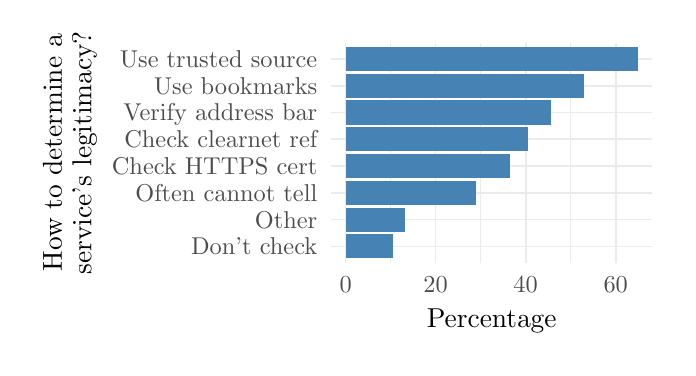
\begin{tikzpicture}[x=1pt,y=1pt]
\definecolor{fillColor}{RGB}{255,255,255}
\path[use as bounding box,fill=fillColor,fill opacity=0.00] (0,0) rectangle (231.26,115.63);
\begin{scope}
\path[clip] (109.60, 30.77) rectangle (225.76,110.13);
\definecolor{drawColor}{gray}{0.92}

\path[draw=drawColor,line width= 0.3pt,line join=round] (131.15, 30.77) --
	(131.15,110.13);

\path[draw=drawColor,line width= 0.3pt,line join=round] (163.68, 30.77) --
	(163.68,110.13);

\path[draw=drawColor,line width= 0.3pt,line join=round] (196.21, 30.77) --
	(196.21,110.13);

\path[draw=drawColor,line width= 0.6pt,line join=round] (109.60, 36.58) --
	(225.76, 36.58);

\path[draw=drawColor,line width= 0.6pt,line join=round] (109.60, 46.26) --
	(225.76, 46.26);

\path[draw=drawColor,line width= 0.6pt,line join=round] (109.60, 55.94) --
	(225.76, 55.94);

\path[draw=drawColor,line width= 0.6pt,line join=round] (109.60, 65.61) --
	(225.76, 65.61);

\path[draw=drawColor,line width= 0.6pt,line join=round] (109.60, 75.29) --
	(225.76, 75.29);

\path[draw=drawColor,line width= 0.6pt,line join=round] (109.60, 84.97) --
	(225.76, 84.97);

\path[draw=drawColor,line width= 0.6pt,line join=round] (109.60, 94.65) --
	(225.76, 94.65);

\path[draw=drawColor,line width= 0.6pt,line join=round] (109.60,104.33) --
	(225.76,104.33);

\path[draw=drawColor,line width= 0.6pt,line join=round] (114.88, 30.77) --
	(114.88,110.13);

\path[draw=drawColor,line width= 0.6pt,line join=round] (147.41, 30.77) --
	(147.41,110.13);

\path[draw=drawColor,line width= 0.6pt,line join=round] (179.95, 30.77) --
	(179.95,110.13);

\path[draw=drawColor,line width= 0.6pt,line join=round] (212.48, 30.77) --
	(212.48,110.13);
\definecolor{fillColor}{RGB}{70,130,180}

\path[fill=fillColor] (114.88, 32.22) rectangle (131.91, 40.93);

\path[fill=fillColor] (114.88, 41.90) rectangle (136.32, 50.61);

\path[fill=fillColor] (114.88, 51.58) rectangle (162.17, 60.29);

\path[fill=fillColor] (114.88, 61.26) rectangle (174.14, 69.97);

\path[fill=fillColor] (114.88, 70.94) rectangle (180.76, 79.65);

\path[fill=fillColor] (114.88, 80.61) rectangle (188.96, 89.32);

\path[fill=fillColor] (114.88, 90.29) rectangle (200.95, 99.00);

\path[fill=fillColor] (114.88, 99.97) rectangle (220.48,108.68);
\end{scope}
\begin{scope}
\path[clip] (  0.00,  0.00) rectangle (231.26,115.63);
\definecolor{drawColor}{gray}{0.30}

\node[text=drawColor,anchor=base east,inner sep=0pt, outer sep=0pt, scale=  0.88] at (104.65, 33.55) {Don't check};

\node[text=drawColor,anchor=base east,inner sep=0pt, outer sep=0pt, scale=  0.88] at (104.65, 43.23) {Other};

\node[text=drawColor,anchor=base east,inner sep=0pt, outer sep=0pt, scale=  0.88] at (104.65, 52.91) {Often cannot tell};

\node[text=drawColor,anchor=base east,inner sep=0pt, outer sep=0pt, scale=  0.88] at (104.65, 62.58) {Check HTTPS cert};

\node[text=drawColor,anchor=base east,inner sep=0pt, outer sep=0pt, scale=  0.88] at (104.65, 72.26) {Check clearnet ref};

\node[text=drawColor,anchor=base east,inner sep=0pt, outer sep=0pt, scale=  0.88] at (104.65, 81.94) {Verify address bar};

\node[text=drawColor,anchor=base east,inner sep=0pt, outer sep=0pt, scale=  0.88] at (104.65, 91.62) {Use bookmarks};

\node[text=drawColor,anchor=base east,inner sep=0pt, outer sep=0pt, scale=  0.88] at (104.65,101.29) {Use trusted source};
\end{scope}
\begin{scope}
\path[clip] (  0.00,  0.00) rectangle (231.26,115.63);
\definecolor{drawColor}{gray}{0.30}

\node[text=drawColor,anchor=base,inner sep=0pt, outer sep=0pt, scale=  0.88] at (114.88, 19.76) {0};

\node[text=drawColor,anchor=base,inner sep=0pt, outer sep=0pt, scale=  0.88] at (147.41, 19.76) {20};

\node[text=drawColor,anchor=base,inner sep=0pt, outer sep=0pt, scale=  0.88] at (179.95, 19.76) {40};

\node[text=drawColor,anchor=base,inner sep=0pt, outer sep=0pt, scale=  0.88] at (212.48, 19.76) {60};
\end{scope}
\begin{scope}
\path[clip] (  0.00,  0.00) rectangle (231.26,115.63);
\definecolor{drawColor}{RGB}{0,0,0}

\node[text=drawColor,anchor=base,inner sep=0pt, outer sep=0pt, scale=  0.99] at (167.68,  7.44) {Percentage};
\end{scope}
\begin{scope}
\path[clip] (  0.00,  0.00) rectangle (231.26,115.63);
\definecolor{drawColor}{RGB}{0,0,0}

\node[text=drawColor,rotate= 90.00,anchor=base,inner sep=0pt, outer sep=0pt, scale=  0.99] at ( 12.32, 70.45) {How to determine a};

\node[text=drawColor,rotate= 90.00,anchor=base,inner sep=0pt, outer sep=0pt, scale=  0.99] at ( 23.01, 70.45) {service's legitimacy?};
\end{scope}
\end{tikzpicture}

    \caption{How our respondents determine an onion service's legitimacy.}
    \label{fig:determining-legitimacy}
\end{figure}


We also asked our interview participants how they knew that the websites they went to were actually the ones that they wanted to go to.  We observed mainly two different patterns – when people relied on someone else and when they tried to work this out on their own. Starting from the first group, the biggest number of interviewees responded that their main strategy for verification of onion links was word of mouth (5) and assistance of someone else while using OS (4) as P03 admitted “ (I) Let people show me them. I don't go there myself.” Also two interview participants relied on trusted resources and two entered OS via their corresponding websites as a way of protection. One of the most often (3 interviewees) approach taken in the second category, was simply checking and comparing URLs to see whether they matched to ‘clear net site’ (P14). Furthermore, two interview participants depend on their own experience, one on http certificate, another one would lower the security settings in order to check the website. There was one interviewee who believed that just using Tor is verification itself and from the other hand, there was one interview participant who simply avoided onion pages.

Our interviewees listed many different strategies which they used to verify the authenticity of Onion links but the biggest number of them (6) stated that they don’t know how to do that and “That’s the whole problem” (P03). Moreover, two interviewees thought it is not even possible.


\subsection{Onion Service Issues \& Improvements}
\label{sec:improve}

\subsubsection{Vanity Domains vs. Phishing Attacks}

The majority of our interview participants (9/17) agreed on the fact that there is a big likelihood of phishing attacks, one of them explained the phenomenon this way: ``the two approaches I know from the normal Web still apply here, which is typo-squatting, registering an .onion that's only a slight variation away, or bit-squatting, which is slightly different, but it involves a single or a few bit flips within an .onion address, so that it looks relatively similar.'' (P06), while another interview participant showed his solution for this problem: ``If you're manually typing it in I suppose they could be a problem, but I primarily cut and paste.'' (P25). In three interviewees the anonymous character of OS raised doubt over their security.

Phishing remains an issue despite onion services' extra anonymity and security
properties.  Past work has documented phishing onion sites that transparently
rewrote Bitcoin addresses to hijack Bitcoin
transactions~\cite{Winter2016a,Nurmi2015a,Monteiro2016a}.  Key to this attack is
the difficulty of telling apart an authentic onion domain from an impersonation.
For conventional domains we rely on (\textsc{ev}) certificates, browser
protections, search results, and long-lived reputation, but none of these
methods have matured for onion services.  Does the nature of onion services
facilitate phishing attacks?  If so, what can we do to mitigate the issue?



Ten out of 17 interviewees found the idea of vanity domains as the big usability improvement: ``In terms of mnemonics and easier recollection if you can chunk words that are associated with daily life and not just a random. If there's entropy in the stream, there's no way I'm going to remember that more than a few characters.'' (P18) and from different perspective, P10 thought of vanity domains as a sort of mapping tool that makes you feel safer and more protected: ``I think that for people who don't spend a lot of time using those types of services, it definitely gives you a more familiar framework for thinking about where you are on the Internet. If people think ... people have a pretty strange geographic metaphors for navigating the internet, but I think this idea of where are you? Well, I'm at this place I can't even name, I can't say it out loud, I think that can be a barrier for people.'' While 1 person, P26, did not find vanity domains practical and seemed to distrust them: ``I don't think it's useful because, you know, only the first ... only some character and it's followed by another random word, so I don't think it's very useful. And phishing can still copy that. They can use more similar upper. I think this not valuable because I think phishing can use a combination (...) I don't think what I can remember is safe now. Even I don't know what my password is or my e-mail is.'' Interestingly, some \adz{how many} survey
respondents consider vanity domains economically unfair because wealthy entities
can afford to generate longer prefixes such as Facebook \mc{explain why in related work}.


What is more interesting, the problem of phishing attacks, that lays in mistyped variation of the real address, and thinking of and proposing vanity domains as possible improvement generates another problem that 8 of our interview participants saw: such improvement could multiple phishing attacks. As P13 elaborated: ``I think in theory, on the one, it makes it easier for you to recognize where you are, it makes it easier for you to perhaps, share the URL or type it out. On the other hand, I've seen concerns that, by having a vanity URL where perhaps people only look for the Facebook portion and they don't pay attention to what comes after it could potentially make it easier to exploit unsuspecting users. Send them a link that also says Facebook but the numbers after it are different, but you just see the Facebook part and go, ``It's fine, it's Facebook.'' That can be a risk to them.''  In addition, P05 simply explained:  ``It seems like it would encourage more trust on behalf of the user, but then again, maybe make phishing easier too, if phishers are making vanity domains themselves. Yeah, that seems like it could go both ways actually.'' Furthermore, one interviewee expressed his concern about onion vanity domains saying that he ``wouldn’t use it for fun'' (P02).
Among our survey respondents there was concern that the
short and recognizable prefixes tempt users to only verify the prefix and ignore
subsequent characters.  One survey respondent reported that \textquote{I only memorize
the first part of the domain.} \mc{need participant id} while another wrote:

\mc{need participant id}
\begin{displayquote}[Survey respondent]
If there isn't some cognizable word at the start, it'll be more difficult for me
to determine if I'm going to the correct domain or a scam. I may end up going to
less .onion sites as a result.
\end{displayquote}

Focusing only on the vanity part of a domain allows attackers to create an
impersonation domain that features the original's prefix but differs in
subsequent characters.  Nurmi~\cite{Nurmi2015a} and
Monteiro~\cite{Monteiro2016a} have both documented such an attack, but its
effectiveness is not known.

Based on the root DNS dataset, we evaluated how often two 
different onion domains are extremely similar to one another; this evaluation can potentially shed 
light on how often an onion domain may be phished.  We first extracted all correctly-formatted 
onion domains from the dataset and then computed a similarity metric between each unique pair of onion 
domains.  Using the Jaro-Winkler string similarity metric, which is the edit distance between two strings and gives more weight 
to strings with common prefixes, we assign a similarity value between \[0,1\], where 0 represents completely different strings 
and 1 represents matching strings, to each unique domain pair. We use this metric because people tend to check the first part of the domain as opposed to the last part. 
Our results show that .007\% (8,672) of all unique domain pairs (119,668,185) have an extremely high similarity ($> .90$); for example, 
\url{bitfog2jzic5tnh7.onion} and \url{bitfog2y7y2pfv75.onion} have a similarity of .917.

Moreover, 6 interviewees reported that one of their issues is correct web page dilemma – you can never be sure whether you are on the right website, three reported that .onion links are easy to mistype and also, one interview participant noticed that onion URL changes randomly. All of these problems led to proposed improvements like stable pattern of words or numbers in URL (3/17) to make it more readable and one interviewee suggested that the URL should be composed without numbers, only with letters - which corresponds to complaint of survey respondents mentioned in \Cref{sec:perception}.

\subsubsection{Onion Services Operations}
We asked our survey respondents if they had ever set up their own onion site and the issues they faced as reported in \Cref{fig:onion-operation-concerns}.  We asked about three potential attacks on onion services; \first~somebody setting up a
phishing site for the operator's site, \second~a denial-of-service attack, and
\third~a deanonymization attack.  More than half of our survey respondents who operated an onion service were at least
somewhat concerned about all of these attacks.  Almost 40\% of survey respondents claimed to be
extremely concerned about somebody deanonymizing their onion service.  Indeed,
many survey respondents lamented the difficulty of protecting onion services from
application-layer deanonymization attacks.  Matic \ea\ demonstrated some of
these issues in 2015~\cite{Matic2015a}.

\begin{figure}[t]
    \centering
    % Created by tikzDevice version 0.10.1 on 2018-02-09 14:59:34
% !TEX encoding = UTF-8 Unicode
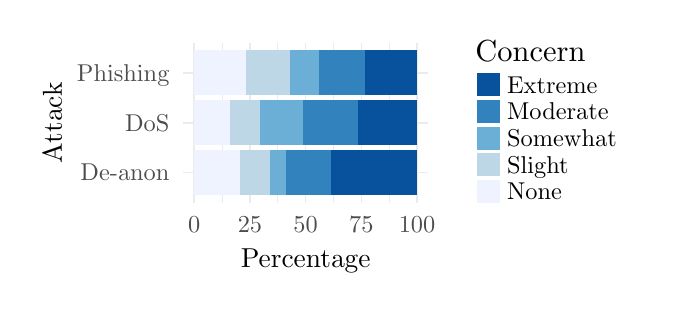
\begin{tikzpicture}[x=1pt,y=1pt]
\definecolor{fillColor}{RGB}{255,255,255}
\path[use as bounding box,fill=fillColor,fill opacity=0.00] (0,0) rectangle (224.04, 93.95);
\begin{scope}
\path[clip] ( 56.18, 30.77) rectangle (144.74, 88.45);
\definecolor{drawColor}{gray}{0.92}

\path[draw=drawColor,line width= 0.3pt,line join=round] ( 70.26, 30.77) --
	( 70.26, 88.45);

\path[draw=drawColor,line width= 0.3pt,line join=round] ( 90.39, 30.77) --
	( 90.39, 88.45);

\path[draw=drawColor,line width= 0.3pt,line join=round] (110.52, 30.77) --
	(110.52, 88.45);

\path[draw=drawColor,line width= 0.3pt,line join=round] (130.64, 30.77) --
	(130.64, 88.45);

\path[draw=drawColor,line width= 0.6pt,line join=round] ( 56.18, 41.59) --
	(144.74, 41.59);

\path[draw=drawColor,line width= 0.6pt,line join=round] ( 56.18, 59.61) --
	(144.74, 59.61);

\path[draw=drawColor,line width= 0.6pt,line join=round] ( 56.18, 77.64) --
	(144.74, 77.64);

\path[draw=drawColor,line width= 0.6pt,line join=round] ( 60.20, 30.77) --
	( 60.20, 88.45);

\path[draw=drawColor,line width= 0.6pt,line join=round] ( 80.33, 30.77) --
	( 80.33, 88.45);

\path[draw=drawColor,line width= 0.6pt,line join=round] (100.45, 30.77) --
	(100.45, 88.45);

\path[draw=drawColor,line width= 0.6pt,line join=round] (120.58, 30.77) --
	(120.58, 88.45);

\path[draw=drawColor,line width= 0.6pt,line join=round] (140.71, 30.77) --
	(140.71, 88.45);
\definecolor{fillColor}{RGB}{239,243,255}

\path[fill=fillColor] ( 60.20, 33.48) rectangle ( 76.78, 49.70);
\definecolor{fillColor}{RGB}{189,215,231}

\path[fill=fillColor] ( 76.78, 33.48) rectangle ( 87.44, 49.70);
\definecolor{fillColor}{RGB}{107,174,214}

\path[fill=fillColor] ( 87.44, 33.48) rectangle ( 93.35, 49.70);
\definecolor{fillColor}{RGB}{49,130,189}

\path[fill=fillColor] ( 93.35, 33.48) rectangle (109.54, 49.70);
\definecolor{fillColor}{RGB}{8,81,156}

\path[fill=fillColor] (109.54, 33.48) rectangle (140.72, 49.70);
\definecolor{fillColor}{RGB}{239,243,255}

\path[fill=fillColor] ( 60.20, 51.50) rectangle ( 73.16, 67.72);
\definecolor{fillColor}{RGB}{189,215,231}

\path[fill=fillColor] ( 73.16, 51.50) rectangle ( 83.77, 67.72);
\definecolor{fillColor}{RGB}{107,174,214}

\path[fill=fillColor] ( 83.77, 51.50) rectangle ( 99.47, 67.72);
\definecolor{fillColor}{RGB}{49,130,189}

\path[fill=fillColor] ( 99.47, 51.50) rectangle (119.50, 67.72);
\definecolor{fillColor}{RGB}{8,81,156}

\path[fill=fillColor] (119.50, 51.50) rectangle (140.71, 67.72);
\definecolor{fillColor}{RGB}{239,243,255}

\path[fill=fillColor] ( 60.20, 69.53) rectangle ( 79.05, 85.75);
\definecolor{fillColor}{RGB}{189,215,231}

\path[fill=fillColor] ( 79.05, 69.53) rectangle ( 94.75, 85.75);
\definecolor{fillColor}{RGB}{107,174,214}

\path[fill=fillColor] ( 94.75, 69.53) rectangle (105.36, 85.75);
\definecolor{fillColor}{RGB}{49,130,189}

\path[fill=fillColor] (105.36, 69.53) rectangle (121.85, 85.75);
\definecolor{fillColor}{RGB}{8,81,156}

\path[fill=fillColor] (121.85, 69.53) rectangle (140.70, 85.75);
\end{scope}
\begin{scope}
\path[clip] (  0.00,  0.00) rectangle (224.04, 93.95);
\definecolor{drawColor}{gray}{0.30}

\node[text=drawColor,anchor=base east,inner sep=0pt, outer sep=0pt, scale=  0.88] at ( 51.23, 38.56) {De-anon};

\node[text=drawColor,anchor=base east,inner sep=0pt, outer sep=0pt, scale=  0.88] at ( 51.23, 56.58) {DoS};

\node[text=drawColor,anchor=base east,inner sep=0pt, outer sep=0pt, scale=  0.88] at ( 51.23, 74.61) {Phishing};
\end{scope}
\begin{scope}
\path[clip] (  0.00,  0.00) rectangle (224.04, 93.95);
\definecolor{drawColor}{gray}{0.30}

\node[text=drawColor,anchor=base,inner sep=0pt, outer sep=0pt, scale=  0.88] at ( 60.20, 19.76) {0};

\node[text=drawColor,anchor=base,inner sep=0pt, outer sep=0pt, scale=  0.88] at ( 80.33, 19.76) {25};

\node[text=drawColor,anchor=base,inner sep=0pt, outer sep=0pt, scale=  0.88] at (100.45, 19.76) {50};

\node[text=drawColor,anchor=base,inner sep=0pt, outer sep=0pt, scale=  0.88] at (120.58, 19.76) {75};

\node[text=drawColor,anchor=base,inner sep=0pt, outer sep=0pt, scale=  0.88] at (140.71, 19.76) {100};
\end{scope}
\begin{scope}
\path[clip] (  0.00,  0.00) rectangle (224.04, 93.95);
\definecolor{drawColor}{RGB}{0,0,0}

\node[text=drawColor,anchor=base,inner sep=0pt, outer sep=0pt, scale=  0.99] at (100.46,  7.44) {Percentage};
\end{scope}
\begin{scope}
\path[clip] (  0.00,  0.00) rectangle (224.04, 93.95);
\definecolor{drawColor}{RGB}{0,0,0}

\node[text=drawColor,rotate= 90.00,anchor=base,inner sep=0pt, outer sep=0pt, scale=  0.99] at ( 12.32, 59.61) {Attack};
\end{scope}
\begin{scope}
\path[clip] (  0.00,  0.00) rectangle (224.04, 93.95);
\definecolor{drawColor}{RGB}{0,0,0}

\node[text=drawColor,anchor=base west,inner sep=0pt, outer sep=0pt, scale=  1.10] at (161.81, 81.72) {Concern};
\end{scope}
\begin{scope}
\path[clip] (  0.00,  0.00) rectangle (224.04, 93.95);
\definecolor{fillColor}{RGB}{8,81,156}

\path[fill=fillColor] (162.52, 69.18) rectangle (170.74, 77.40);
\end{scope}
\begin{scope}
\path[clip] (  0.00,  0.00) rectangle (224.04, 93.95);
\definecolor{fillColor}{RGB}{49,130,189}

\path[fill=fillColor] (162.52, 59.55) rectangle (170.74, 67.76);
\end{scope}
\begin{scope}
\path[clip] (  0.00,  0.00) rectangle (224.04, 93.95);
\definecolor{fillColor}{RGB}{107,174,214}

\path[fill=fillColor] (162.52, 49.91) rectangle (170.74, 58.12);
\end{scope}
\begin{scope}
\path[clip] (  0.00,  0.00) rectangle (224.04, 93.95);
\definecolor{fillColor}{RGB}{189,215,231}

\path[fill=fillColor] (162.52, 40.27) rectangle (170.74, 48.49);
\end{scope}
\begin{scope}
\path[clip] (  0.00,  0.00) rectangle (224.04, 93.95);
\definecolor{fillColor}{RGB}{239,243,255}

\path[fill=fillColor] (162.52, 30.64) rectangle (170.74, 38.85);
\end{scope}
\begin{scope}
\path[clip] (  0.00,  0.00) rectangle (224.04, 93.95);
\definecolor{drawColor}{RGB}{0,0,0}

\node[text=drawColor,anchor=base west,inner sep=0pt, outer sep=0pt, scale=  0.88] at (173.26, 70.26) {Extreme};
\end{scope}
\begin{scope}
\path[clip] (  0.00,  0.00) rectangle (224.04, 93.95);
\definecolor{drawColor}{RGB}{0,0,0}

\node[text=drawColor,anchor=base west,inner sep=0pt, outer sep=0pt, scale=  0.88] at (173.26, 60.62) {Moderate};
\end{scope}
\begin{scope}
\path[clip] (  0.00,  0.00) rectangle (224.04, 93.95);
\definecolor{drawColor}{RGB}{0,0,0}

\node[text=drawColor,anchor=base west,inner sep=0pt, outer sep=0pt, scale=  0.88] at (173.26, 50.99) {Somewhat};
\end{scope}
\begin{scope}
\path[clip] (  0.00,  0.00) rectangle (224.04, 93.95);
\definecolor{drawColor}{RGB}{0,0,0}

\node[text=drawColor,anchor=base west,inner sep=0pt, outer sep=0pt, scale=  0.88] at (173.26, 41.35) {Slight};
\end{scope}
\begin{scope}
\path[clip] (  0.00,  0.00) rectangle (224.04, 93.95);
\definecolor{drawColor}{RGB}{0,0,0}

\node[text=drawColor,anchor=base west,inner sep=0pt, outer sep=0pt, scale=  0.88] at (173.26, 31.71) {None};
\end{scope}
\end{tikzpicture}

    \caption{The level of concern onion service operators have with respect to a
    phishing clone of their service, denial-of-service attacks, and
    deanonymization.}
    \label{fig:onion-operation-concerns}
\end{figure}

One of our interviewee, P16, explained encryption technology issues, his wish to secure his content but also his positive attitude towards the future of onion services: „As far as other websites, I do have some sites that I want to run, but I'm just waiting for the encryption technology to become better, and I don't think we're that far off it, as in we're talking months. (…) another thing about onion services, is whether or not those hosts are actually encrypted, and that the data that you actually post on those things is also encrypted, so if they are actually taken down by third parties for whatever reason, that you can say, "Well it doesn't matter the site's gone, but my stuff's pretty much safe, because I have my own key."“

Another problems that our interview participants listed were browser fingerprinting (2), as well as changing domain problem, when one site is taken down and its domain is changed it is hard to find it (1). There was also one interviewee who claimed that his problem lies in remembering where the exact domain was but one person saw no domain format problems. Furthermore, participant P01 had a problem with a Firefox  browser regarding onion links – it did not recognize .onion domains as being secure. 

Interestingly, most (83\%) of our survey participants did not expect the
next-generation domain format to change their browsing habits because they treat onion domains as
opaque identifiers and handle these links via tools such as bookmarks.  For the 17\% who expressed concern over the next generation domain format \mc{can we define what this is?}, they felt that they would no longer be able to memorize even the small
number of onion domains (such as Facebook's) that they used.
 This suggests that although onion links are difficult to handle, usability may not worsen with the new domain format.


\subsubsection{User Experience Design}


Many survey respondents had performance concerns when it comes to onion services. \mc{need participant id}  One survey user stated, ``I would
always prefer the onion site, but for video sites like YouTube I would likely
often use the normal site to be able to get a higher quality stream due to
higher bandwidth.'' Another drawback of OS was identified in the latency and according to 3 interview participants the access time was too slow. 

Other survey respondents mentioned not wanting to log in to onion sites
because they believe it defeats the purpose by revealing private data---a fallacy that we discussed in
\Cref{sec:perception}.  Our interviewees mentioned a lot technical improvements that they would like to see. Four of them put the emphasis on importance of creating valid search engine type tool, while two interviewees would like to see safe bookmarking tool.  Three interviewees wanted CAPTCHAs to be gone and one interview participant wanted login facility as well as to see some authentication to be added to onion sites. 

Moreover, another interviewee thought that OS should be safer but they should preserve anonymity at the same time. When it come to anonymity, participants listed such possible improvements as anonymous video calls (1), email (1) and file sharing (1). Two interview participants mentioned that faster access time to websites would be a feature they would like to see. From a different perspective, two interviewees wished there would be a way to automatically redirect to onion services while using Tor and furthermore, one person thought that there should be auto-redirect to Tor, whenever typing onion links, even in a different browser. In addition to that, we asked survey respondents if they would want Tor Browser to automatically redirect them from
a normal web site to its corresponding onion site (\eg, from facebook.com to
facebookcorewwwi.onion). Survey respondents were largely
in favor of this feature:37.78\% said they would always use it, 34.91\% said
they would use it for some sites, 15.61\% said they would never use that feature,   and
11.70\% chose ``Other.'' Survey respondents reported that they liked the convenience of being redirected.
The naysayers were quite passionate, though, and they were concerned about
potential security issues. One respondent said, \mc{participant id needed}
\textquote{What's to stop them from man in the middle'ing me, either by choice,
at the behest of some nefarious entity, or after being hacked?}
We conclude that there is clear interest in such an ``upgrade'' feature provided
that it is carefully designed and offers users an option to control the process
on a per-site basis.


\subsubsection{Education, Accessibility \& Knowledge}

One of the biggest issues for participants was the fact that onion sites are hard to find (5/17): “In my line of work, people talk about, "You can get all sorts of things on the dark web. There's all sorts of things, marketplaces where things are bought and sold or all sorts of information you can find." But unless you know, if I want to find out, what are all of the forums where people sell credit card data? I would have to rely on someone who has previously collated the directory of that sort of stuff. I think that would be the main thought I'd have is how do you discover that? How do you find stuff if you don't know what you're looking for or only have a vague idea? (P13) and for one interviewee onion links were also hard to share.  In addition to that, one participant wished to be able to find Onion Links through “normal” browsers. 

Among the survey respondents who were not satisfied with how they discover onion services (40%), the most
prominent complaint was about link rot on aggregators.  There is significant
churn among onion sites, and our respondents were frustrated that aggregators
are typically not curated and therefore link to numerous dead domains.  The lack
of curation also leads to these aggregators' containing the occasional scam and
phishing site.  The difficulty of telling apart two given onion domain names
exacerbates this issue for users.  Another common wish for aggregators was for
them to be more verbose in their description of onion sites.  In particular,
some survey respondents wanted to avoid illegal and pornographic content, which is often
difficult if the description is vague and the onion domain reveals nothing about
its content.  Many survey respondents were not aware of search engines such as Ahmia.
Among those survey respondents that were aware of such engines, many were dissatisfied with both the search results and
the number of indexed onion sites.  Unsurprisingly, a ``Google for onion sites''
was a frequent wish.


Moreover, 7 interviewees wished that OS would be simply more accessible for everybody, not only in work but also in every other aspect of our lives, for example in having an access to social media or even planning a wedding with friends on Signal - P10 elaborated: ``A lot of it is about adoption. I feel like it's important to normalize the use of these tools outside of this world to people and just to sort of, in groups of friends or colleagues or whatever (...) Communication is not always top secret and hardcore, sometimes it's fun. If people are doing their fun communication one place and their serious communication in another, then there's lots of security problems with that.'' 

We also asked our survey respondents if they would prefer onion versions of popular web sites such as
YouTube, Twitter, or Amazon to their normal web
sites. 49.07\% of survey respondents said they
would always prefer the onion site, 30.72\% chose ``Other'' and 20.21\% of
respondents said they would always prefer the normal web site. As a further matter, 3 interviewees wished to see big popular domains having OS, which P06 explained and brought up different aspect of such change: ``I think a lot of people would enjoy being more anonymous in some of those spaces. I also think that would have an effect on the culture of those spaces, and it would change. That's not necessarily a good or bad thing, it's just that you behave differently in a space where everyone is anonymous, or if everyone's not anonymous. But in mixed spaces, where some people are and some people aren't, there are some interesting culture clashes.'', but also, one interviewee thought that not only big domains, but every website should have its correspondent onion site. In addition, any survey respondents expressed frustration about the difficulty of finding out if a particular website, such as 
``example.com'' has a corresponding onion service.  A common wish was to have
a website list its onion service prominently in a footer.  Ironically, some
survey respondents were surprised that torproject.org has a corresponding onion
site---they could not find it on the web site.


 On the other hand, one person wished to see more ``practical'' for general public related content rather than Facebook; websites that would be safe for example for activists to use or ``For instance, any kind of website that gives Chinese dissidents access to information about how to go around a firewall. Much more applied, like that.'' (P07)

Finally, the possible improvement that was mentioned most often by our participants was education about onion services (7/17). Our interviewees seemed concern about not enough resources that they could find to learn how to use OS in secure way and even know what OS are. Furthermore, as P07 pointed out, OS are not as popular as they could be: „I think usability is one part. I think. I'm not so much concerned, actually, about the onion services being improved, 'cause I think you guys do a very good job. My concern is more about getting this out to people who aren't in this space, communicating what that is, making sure that there's more uptake of it.“
 Some wanted to know how to use onion service correctly and stop being uncertain about its properties: ``Like really clear user education in the installation process would be great for people like me and for people [...] like me, who are like ``Okay, this is a thing I can use, why am I using it again? What am I using it for? What does it do?'' And why would it potentially even be breaking these other apps. I'm I being watched and now my phone is being destroyed. Or is it like a simple technical problem, that can be overcome? (P08). One of our interviewee thought that bulletin would be a good idea, while 2 thought that there should be some websites that would help and inform people about usage of OS – also, according to one interview participant, the fact that there was no support center was a big problem related to OS. 
The lack of proper education accompanies by a phenomenon, which 3 of our participants called ``cultural mysticism''. Since people do not have extended (and sometime even little) knowledge about OS, they tend to misinterpret some information about them, as P10 explained: „the perception that these are hardcore security tools sometimes signals to ordinary users that they are also difficult or badly designed or complicated to use, and that's not really the case with Tor“, but also they may be even afraid to use them, as P08’s opinion mentioned before: Because it's also super scary. Like you think you're playing with this spy thing [...] Sometimes it's actually a really simple technical thing that's not terrifying. And to like demystify those kind of things would be really nice.“. This also led to suggested improvement to have directory ordered by categories that would make usage of OS simpler (3/17) since there was also one interviewee who wished that OS would be easier to use. Moreover, one interviewee proposed warnings to alert when something goes wrong, for example the site that one would like to enter might deanonymize the user. Also, there was one interviewee who felt under qualified to answer what kind of improvements he would like to see in OS.
